  % !TeX root = ../libro.tex
% !TeX encoding = utf8

\chapter{Introducción}\label{ch:pv-introduccion}

La \textbf{selección de modelos} es una tarea muy importante en la resolución de problemas del aprendizaje automático (y profundo) ya que de entre varios modelos propuestos como solución querremos escoger el mejor.

Para valorar esto recurrimos a las \textbf{métricas}, aplicaciones que miden cuantitativamente, usando algún criterio, la semejanza entre la función $f$ que estamos intentando aprender y la función $h$ aprendida por el modelo.

Usando una métrica podemos comparar los resultados entre distintos modelos y escoger el que mayor valor arroje, sin embargo aquí entra el problema de la \textbf{validación}. Si solo nos basamos con el resultado de la métrica en el mismo conjunto donde hemos entrenado los datos, puede que estemos sobrestimando bastante el valor real debido al efecto del \textbf{sobreajuste}.

Recordemos que este efecto se daba cuando el modelo se ajustaba demasiado a los datos de la muestra actual obteniendo un sesgo muy bajo, sin embargo, vimos que también la varianza aumentaba mucho, provocando que para otra muestra distinta de la distribución el modelo obtuviese un rendimiento mucho peor al de la muestra donde fue entrenada.

Por esta razón es necesaria una manera más realista de medir los modelos para evitar el sobreajuste, surgiendo así la \textbf{división clásica} entrenamiento/test. Este método consiste en, o bien obtener dos muestras independientes de la distribución o dividir una única muestra en dos antes de manipular los datos. La muestra de entrenamiento se usa para entrenar el modelo y la muestra de test para valorar los modelos, ya que es una nueva muestra que no ha visto el modelo anteriormente.

Aunque este método ya resuelva nuestro problema también se puede querer hacer la selección de los modelos antes de realizar la valoración en el conjunto de test para, por ejemplo, quedarnos con un subconjunto menor de modelos de un gran número de modelos considerados para reducir tiempo de cómputo innecesario. También entra aquí la \textbf{selección de hiperparámetros} que es una selección de modelos solo que considerando el mismo modelo base y lo que cambia entre modelos es algún hiperparámetro (por ejemplo el número de neuronas en una red neuronal).

Para resolver esto hay generalmente dos alternativas: hacer una partición más del conjunto de entrenamiento, quedándonos en total con el de entrenamiento, test y el de \textbf{validación}; o bien utilizar el método de \textbf{validación cruzada}.

La validación cruzada consiste en dividir la muestra de entrenamiento en $k$ conjuntos del mismo tamaño y repetir $k$ veces la validación usando un conjunto como \emph{test} y el resto de entrenamiento. Este método intenta dar un valor más robusto que usando un único conjunto de validación, y además puede indicar una idea de cómo de variable será en función a la varianza de los resultados.

Estos son los métodos clásicos que se han usado generalmente para obtener valores de la métrica realistas y que nos permiten comparar modelos y por tanto, elegir los mejores en base a esto. Sin embargo, esta clase de validaciones confía que en las muestras de datos recogidas de la distribución es \textbf{suficientemente representativa} de la distribución subyacente, y que han sido recogidos \textbf{sin sesgo} alguno \cite{zhang2019perturbation}.

Estos problemas se puede presentar perfectamente cuando el problema es muy grande y es muy difícil obtener muchas muestras, o cuando se ha cometido algún error al tomar las muestras que nadie se ha percatado. Por ejemplo, en la detección de caras en imágenes, debido a la gran cantidad de posibilidades de formas en las que podrían estar, se necesita una muestra muy grande que abarque múltiples y diversas maneras para poder tener una representación buena de la distribución y además que no haya sesgos (solo salen caras en fotos con buena iluminación, o de gente con tez blanca...).

Por estas razones se presenta un nuevo método para valorar modelos basado en una heurística: $PV$ (\emph{Perturbated Validation}) \cite{zhang2019perturbation}. Este método \textbf{no} utiliza las mismas técnicas clásicas de utilizar un conjunto aparte sino que considera todo el conjunto entero, sin divisiones. En lineas generales trata de valorar si el modelo ha entendido realmente \textbf{la relación subyacente de los datos} midiendo como varía el comportamiento del modelo frente a \textbf{perturbaciones graduales} en los datos.

Nuestro objetivo será ver el funcionamiento de esta heurística, su comportamiento en casos reales, mediante una experimentación utilizando muchos modelos y conjuntos de datos para observar y analizar si nos resulta de utilidad y puede aportar algo nuevo en el paradigma actual de selección de modelos.

\chapter{Selección de modelos}\label{ch:pv}

Planteamos el problema de la selección de modelos para problemas de clasificación multiclase en dominios de series temporales: sea $M \in \N$ la longitud de cada serie temporal, $N$ el número de series temporales, $n$ el número de clases y $k$ el número de modelos a ajustar, consideramos el espacio $\mathcal{X} \times Y \subseteq R^m \times \{0, 1, \ldots, n - 1\} $ del que se obtiene una muestra $(X, \textbf{y}) \in \mathcal{X}^N \times Y^N$ (datos $X$ y etiquetas $\textbf{y}$) que sigue una distribución de probabilidad $\mathcal{P}$ desconocida. Sean también el espacio de hipótesis de los modelos considerados $\mathcal{H} = \{\mathcal{H}_1, \ldots, \mathcal{H}_k\}$ de los que se ha obtenido una función cada uno $h_i \in \mathcal{H}_i, \, i = 1, \ldots, k$ que intentan aproximar a la función de etiquetado $f$ definida por:

\begin{align*}
  f : \mathcal{X} & \to Y \\
  \textbf{x} & \mapsto f(\textbf{x}) \in \{0, 1, \ldots, n-1\}.
\end{align*}

Se pide valorar bajo un criterio determinado la aproximación de las funciones de hipótesis a la función de etiquetado (valorar $f \approx h_i$) de manera que se establezca un orden entre los modelos, permitiéndonos seleccionar los modelos con mejor valoración bajo este criterio.

\section{Selección clásica}

Consideramos la selección de modelos clásica: primero tomamos la muestra o \emph{dataset} $(X, \textbf{y})$ de la realizamos una partición en un conjunto de entrenamiento (\emph{train}) y test usando la proporción usual de 80/20\% respectivamente, manteniendo la proporción de clases. Después realizaremos el método de Validación Cruzada con $k$ \emph{pliegues} (\emph{Cross Validation with $k$ folds}, $k$-CV) \cite{stone1974cross} en el conjunto de entrenamiento: como explicamos previamente, consiste en dividir el conjunto de entrenamiento en $k$ subconjuntos de tamaño igual que mantienen la proporción de clases y repetir $k$ veces la validación usando un subconjunto como test y el resto como entrenamiento (\autoref{fig:cv}, \cite{niu2018rfamyloid}).

\begin{figure}[htbp]
  \centering
  %\hspace*{-2.5cm}
  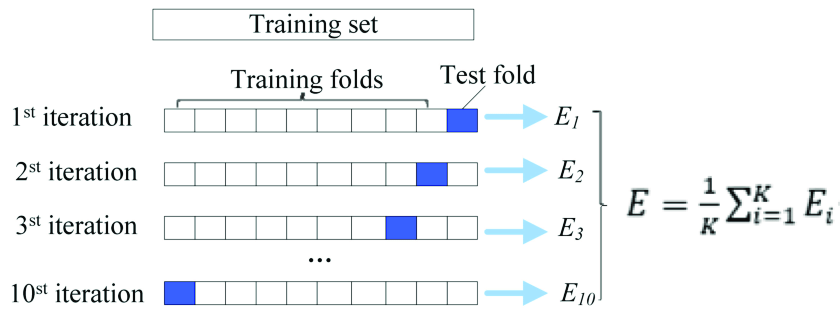
\includegraphics[width=.8\textwidth]{cv}
  \caption{Funcionamiento de la validación cruzada.}
  \label{fig:cv}
\end{figure}


La validación en este caso consiste en entrenar el modelo en el subconjunto de entrenamiento y obtener el valor de la métrica en el subconjunto test; una vez se obtienen los $k$ valores de la métrica se toma el valor final como la media de los valores aunque también se suele devolver la desviación típica o la varianza para tener una idea de cómo puede variar este valor (en qué intervalo de confianza se mueve la métrica).

Para problemas de clasificación consideraremos la métrica \emph{accuracy} $acc$ que ya vimos en \autoref{ch:metricas} que básicamente mide el porcentaje de etiquetas predichas correctamente. Utilizando esta métrica junto a la validación cruzada para cada modelo se obtendrá $acc_{CV}$, y en base a este valor podremos hacer la selección de modelos tomando en cuenta que es un estimador de la métrica en el conjunto test $acc_{test}$; por tanto lo esperable es que el mejor $acc_{CV}$ será probablemente el mejor $acc_{test}$.

\section{Perturbated Validation}

\subsection{Funcionamiento}

La idea general del $PV$ es ir midiendo la métrica $acc$ del modelo conforme se van añadiendo perturbaciones graduales en función de una ratio de error $r$ en la muestra de datos, tomando el valor del $PV$ como el valor absoluto de la \textbf{pendiente} de la recta de regresión con los puntos formados por las tasas de acierto y error $(acc, r)$.

En otras palabras, crearemos $n$ conjuntos copiando las etiquetas originales y cada conjunto con un $r$\% de etiquetas cambiadas. El modelo se entrena por separado con cada conjunto de etiquetas perturbadas y evaluando la métrica en el mismo conjunto, obteniendo así $n$ valores del $acc$ distintos. Es importante entender que el modelo no se reentrena, es como si copiásemos $n$ veces el modelo y cada uno se entrenase y evaluase en un conjunto distinto \textbf{independientemente}.

Teniendo ahora $n$ puntos $\{(r_1, acc_1), \ldots, (r_n, acc_n)\}$ ordenados por $r_1 < \ldots < r_n$ que podemos representar en $\R^2$, usamos regresión lineal para intentar ajustar una recta a los puntos lo mejor posible. El $PV$ entonces será simplemente el valor absoluto de la pendiente de esta recta.

Si el modelo es bueno y capta bien la relación de los datos con las etiquetas entonces no debería ser \emph{engañado} por las etiquetas mal puestas. Esto implica que cuando las etiquetas están casi sin alterar el modelo obtiene un $acc$ muy alto, pero conforme aumentan las perturbaciones el $acc$ va bajando. Entonces al hacer la regresión lineal obtendremos una recta con una pendiente muy pronunciada que se traduce en un $PV$ alto.

Si por el contrario el modelo es muy complejo y se ajusta demasiado a los datos, provocando \textbf{sobreajuste}, entonces obtendrá valores de $acc$ muy altos en todos los casos. La recta de regresión obtenida será muy horizontal y por tanto, con un $PV$ casi nulo. Finalmente, si la complejidad del modelo es insuficiente para captar los datos obtendrá $acc$ muy bajos, variando muy poco y obteniendo una recta horizontal también (\autoref{fig:ej-pv} \cite{zhang2019perturbation}).

\begin{figure}[htpb]
  \centering
  %\hspace*{-2.5cm}
  %\vspace*{-1.5cm}
  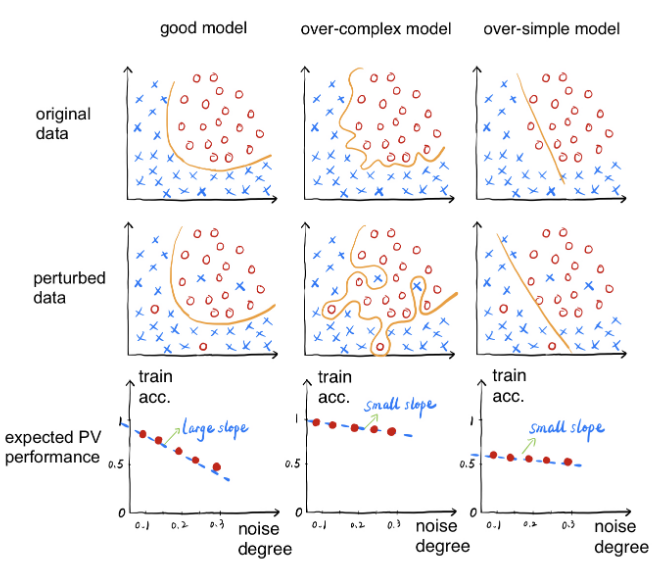
\includegraphics[width=0.8\textwidth]{ej_pv}
  \caption{Idea general de funcionamiento del $PV$.}
  \label{fig:ej-pv}
\end{figure}

Así, el $PV$ intenta medir la correspondencia entre la función de etiquetado real con la aprendida a partir del modelo y del que se esperan dos consecuencias:

\begin{itemize}
  \item Para un valor muy alto la función aprendida $h$ debe ser muy parecida a $f$ y por tanto debería tener valores muy altos de $acc$ en cualquier conjunto.
  \item Para un valor muy bajo la función no se parece, donde pueden pasar dos cosas:
    \begin{itemize}
      \item Si $acc_{train}$ es bajo, entonces es que el modelo tiene un ajuste directamente malo y en $acc_{test}$ también lo será.
      \item Si $acc_{train}$ es alto, entonces el modelo probablemente ha sobreajustado los datos y se tenga que $acc_{test}$ sea mucho menor y haya una gran diferencia con $acc_{train}$.
    \end{itemize}
\end{itemize}

Sin embargo, puede haber casos en los que tengamos un $PV$ bajo y obtengamos $acc_{test}$ bastantes altos, esto es consecuencia de cómo sean las muestras obtenidas de la distribución desconocida, si tienen alguno de los problemas que hemos mencionado (sesgo o representatividad insuficiente) entonces no se verá reflejado el problema en el conjunto de test y los modelos funcionarán igual de bien.

Veamos esto con un ejemplo de \cite{zhang2019perturbation} \autoref{fig:pv-decision} donde se han creado tres \emph{datasets} sintéticos con unas funciones de etiquetado bien definidas, en forma de lunas, círculos y lineal, y se han entrenando con distintos modelos obteniendo tres valores de las métricas utilizadas, PV ($PV$), CV ($acc_{CV}$) y TA ($acc_{test}$) junto con la funciones aprendidas de cada modelo (se corresponde el valor de la etiqueta con un color).

\begin{figure}[htpb]
  \centering
  \hspace*{-1.cm}
  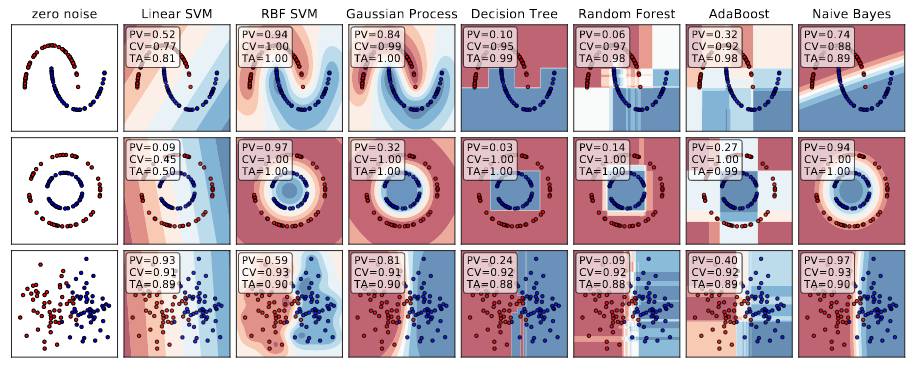
\includegraphics[width=1.2\textwidth]{pv_decision}
  \caption{Tres funciones distintas de clasificación con varios modelos, recogiendo $PV$, $acc_{CV}$ y $acc_{test}$ y la función aprendida.}
  \label{fig:pv-decision}
\end{figure}

Observando los valores PV vemos cómo son mucho más altos cuando la función aprendida del modelo se corresponde con la \emph{forma} original de la función y esto se corresponde con valores casi perfectos de CV y TA. Por otro lado, se asignan valores bajos de PV para los modelos con funciones con una forma más complicada (Random Forest por ejemplo) o cuando no es capaz de captar bien la relación de los datos (Linear SVM), aunque en el primer caso se sigue teniendo valores casi perfectos de CV y TA reflejando lo que habíamos comentado previamente.

Desde luego entre varios modelos con valores CV en torno a 1 podríamos hacer otra selección con quien tenga un mayor valor de PV ya que preferimos quedarnos con un modelo que lo hace igual de bien que el resto pero la función que ha aprendido se adapta mucho más a la \textbf{distribución real de los datos}.

\subsection{Definición}

Sea $r \in [0, 1]$ el ratio de etiquetas perturbadas para cada clase (para mantener las distribución), consideramos una sucesión creciente de ratios $\{r_i\}_{1 \leq i \leq n}$ e $\textbf{y}_{r_i}$ el conjunto de etiquetas con un $r_i$ porcentaje de etiquetas perturbadas por clase. Finalmente notamos $acc(S)$ como el máximo valor de la métrica obtenido con $\mathcal{H}$ en $S = (X, \textbf{y}_{r_i})$, es decir \eqref{eq:acc_rel} \cite{zhang2019perturbation}.

\begin{equation}
  acc(S) = \max_{h \in \mathcal{H}} acc(h) \text{, con } S = (X, \textbf{y}_{r_i}).
  \label{eq:acc_rel}
\end{equation}

Con todos estos elementos ya podemos definir formalmente la heurística $PV$ (\autoref{def:pv}, \cite{zhang2019perturbation}).

\begin{definicion}[Perturbated Validation]\label{def:pv}
  $PV$ es el valor absoluto del coeficiente de la regresión lineal (la pendiente) entre la variable independiente, ratio de etiquetas perturbadas $r_i$, frente la variable dependiente, acierto en el \emph{dataset} perturbado $acc(S_{r_i})$, es decir,

  $$PV = \Bigg|\dfrac{\sum \limits^n_{i = 0} (r_i - \overline{r})(acc(S_{r_{i}}) - \overline{acc(S_r)})}{\sum \limits^n_{i = 0}(r_i - \overline{r})^2}\Bigg|.$$
\end{definicion}

\subsection{Implementación}

Se ha implementado en una clase en \emph{Python} denominada \textbf{$PV$} que nos permite evaluar los modelos usando la descripción mencionada anteriormente. La documentación se puede encontrar en \autoref{ap:documentacion}, aunque merece la pena describir el algoritmo general con pseudocódigo: \autoref{alg:create_pv} para crear los conjuntos de etiquetas perturbados y \autoref{alg:calc_pv} para calcular el $PV$ para un modelo dado.

\begin{algorithm}[htbp]
\SetAlgoLined
 \tcp{Inicializamos los ratios de error}
 \For{$i = 1, \ldots, n$}{
   $r_i \gets err_{ini} + (i - 1) \cdot \dfrac{err_{fin} - err_{ini}}{n - 1}$\;
 }
 \tcp{Para cada ratio creamos unas etiquetas perturbadas}
 \For{$i = 1, \ldots, n$}{
   \tcp{Copiamos las etiquetas originales}
   $\textbf{y}^{(i)} \gets \textbf{y}$\;
   \tcp{Perturbamos para cada clase}
   \For{$j = 1, \ldots, n_{clases}$}{
    \tcp{Perturbamos el \% respecto el número de etiquetas de esa clase}
    $n_{per} \gets r_i \cdot \sum \limits^{|\textbf{y}|}_{k = 1} [[y_k = j]]$\;
    \tcp{Hacemos una permutación de los índices de la clase para escogerlos aleatoriamente}
    $\sigma \gets Permutacion\left( \{ i \in \N : y_i = j\}\right)$\;
    \tcp{Para cada índice se le pone una clase aleatoria distinta de la original}
    \For{$k = 1, \ldots, n_{per}$}{
     $\textbf{y}^{(i)}_{\sigma(k)} \gets Aleatorio(\{1, 2, \ldots, j - 1, j + 1, \ldots, n_{clases}\})$\;
    }
   }
 }
 \KwResult{$r_1, \ldots, r_n$, $\textbf{y}^{(1)}, \ldots, \textbf{y}^{(n)}$}
 \caption{$PV$($\textbf{y}$, $n$, $err_{ini}$, $err_{fin}$)}
 \label{alg:create_pv}
\end{algorithm}

\begin{algorithm}[htbp]
\SetAlgoLined
 \tcp{Para cada conjunto entrenamos el modelo y obtenemos el \emph{accuracy}}
 \For{$i = 1, \ldots, n$}{
  $modelo_{copia} \gets $ copiar($modelo$)\;
  $modelo_{copia}$.fit($X$, $\textbf{y}^{(i)}$)\;
  $acc_i \gets modelo_{copia}$.score($X$, $\textbf{y}^{(i)}$)\;
 }
 \tcp{Calculamos las medias de los errores y el \emph{accuracy}}
 $\overline{r} \gets \dfrac{1}{n} \sum \limits_{i = 1}^{n} r_i$\;
 $\overline{acc} \gets \dfrac{1}{n} \sum \limits_{i = 1}^{n} acc_i$\;
 \tcp{Calculamos el $PV$}
 $PV \gets \Bigg|\dfrac{\sum \limits^n_{i = 0} (r_i - \overline{r})(acc_i - \overline{acc})}{\sum \limits^n_{i = 0}(r_i - \overline{r})^2}\Bigg|$\;
 \KwResult{$PV$}
 \caption{Calcular-$PV$($modelo$, $X$, $\textbf{y}^{(1)}, \ldots, \textbf{y}^{(n)}$, $r_1, \ldots, r_n$)}
 \label{alg:calc_pv}
\end{algorithm}

Para crear los \emph{datasets} perturbados tomamos los errores de manera que sean \textbf{equidistantes}, por lo que solo hace falta pasar como argumento el número de perturbaciones deseadas $n$, y los errores de inicio y fin $err_{1}$ y $err_{n}$. A la hora de elegir los índices aleatoriamente se toman de manera que todos sean \textbf{diferentes} y de la clase correspondiente en el bucle. La clase que se escoge también se asegura que no sea la que tiene actualmente, de manera que la serie tenga efectivamente una \textbf{etiqueta distinta} asociada. Devolvemos las etiquetas perturbadas $Y_i$ como los índices de error $r_i$ necesarios para calcular el $PV$.

Para obtener el $PV$ introducimos el modelo con el resultado del algoritmo anterior, obteniendo un $acc_i$ asociado con cada entrenamiento y medición de rendimiento del modelo (notar que se copia el modelo para que se entrene desde cero). Finalmente obtenemos el $PV$ para el modelo pasado.

\chapter{Experimentación}\label{ch:pv-experimentacion}

En este capítulo vamos a realizar un experimento empírico para investigar la eficacia del $PV$ en problemas de selección de modelos. Para ello consideraremos una serie de modelos usuales utilizados para clasificación, incluyendo un modelo basado en redes LSTM, que entrenaremos en múltiples conjuntos de series temporales, midiendo tanto $PV$ como las medidas clásicas. En base a los resultados haremos un análisis del efecto de esta nueva herramienta.

\section{Modelos}

Enumeramos y explicamos brevemente los distintos modelos utilizados en la experimentación. En el primer estudio usaremos una serie de modelos con hiperparámetros fijos donde se comentan más detalladamente los que se escogen, aunque se volverán a mencionar en la siguiente parte. Para el segundo se probará a encontrar la mejor configuración de hiperparámetros para cada modelo, por lo que se indicará en cada caso que se irá variando.

\subsection{LSTM}

Como tenemos que crear una arquitectura para clasificación en muchísimos \emph{datasets} para comprobar la selección tampoco nos preocuparemos demasiado por sacar el mayor rendimiento posible, así que realizamos un diseño simple pero funcional. Hemos implementado la clase en \emph{Python}.

Utilizando la misma idea que en las redes convolucionales, extraemos características usando una convolución $1$-D de 64 filtros (de salida) y tamaño de núcleo 8 y función de activación ReLU junto a una capa MaxPooling1D con tamaño de núcleo 4 para reducir la dimensión. Después aplicamos una capa LSTM de 80 células quedándonos con el ultimo estado devuelto, junto a una capa Densa de 300 neuronas con activación ReLU que incluye \emph{BatchNormalization} y \emph{Dropout} (técnicas de regularización) donde llegamos finalmente a la última capa de clasificación con $n$ neuronas y activación softmax, siendo $n \in \N$ el número de clases del problema (\autoref{fig:model-select}).

\begin{figure}[htbp]
  \centering
  %\hspace*{-2.5cm}
  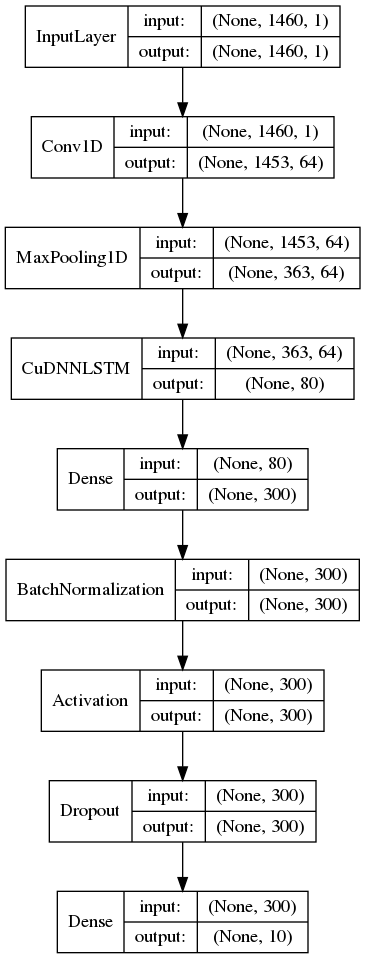
\includegraphics[width=.5\textwidth]{model_select}
  \caption{Arquitectura del clasificador LSTM con series de longitud 1460 y 10 clases.}
  \label{fig:model-select}
\end{figure}

Minimizamos mediante \textbf{ADAM} (modificación de SGD) la función de pérdida \textbf{entropía cruzada categórica} (\emph{categorical crossentropy}, \autoref{def:crossentropy}) que se encarga de medir la diferencia entre dos distribuciones de probabilidad discretas; en nuestro caso estamos aprendiendo la probabilidad de asignar a cada clase que queremos que sea casi 1 para la etiqueta asignada.

\begin{definicion}[Entropía cruzada categórica]
  Sea $n$ el número de clases e $\textbf{y}$ el vector de probabilidades real, dado $\hat{\textbf{y}}$ el vector de probabilidades obtenido por un modelo, la entropía cruzada categórica es una función $E : [0, 1]^n \to \R$ definida por:

  $$ L(\hat{\textbf{y}} ; \textbf{y}) = \sum \limits^n_{i = 1} y_i \log(\hat{y}_i).$$
  \label{def:crossentropy}
\end{definicion}

El entrenamiento se hará durante 300 épocas, con un tamaño de \emph{batch} de 128, usando un 10\% de los datos para el conjunto de validación y añadiendo una parada temprana cuando el $acc_{val}$ no mejore un $0.1$ en 50 épocas, guardando los pesos con mejor resultado.

Esta configuración permite ser relativamente flexible para diferentes \emph{datasets} ya que dejamos muchas épocas para datos más complejos, y una parada temprana para cuando no haya mejora en los simples.

\subsection{SVM}

Las Máquinas de Soporte Vectorial (\emph{Support Vector Machine}, SVM) \cite{cortes1995support} implementadas en \emph{Python} por la librería \emph{scikit-learn} en \cite{scikit2020svm}. Este método se encarga de buscar el mejor hiperplano que \textbf{separe} los datos por sus clases, entendiendo como mejor el que deje a \textbf{más distancia} los puntos más cercanos (siendo estos los puntos de soporte) que tenga ya que este modelo generalizará mejor y por tanto tendrá menor \textbf{sobreajuste} (\autoref{fig:ej-svm} \cite{JavaTpointSVM}).

\begin{figure}[htbp]
  \centering
  %\hspace*{-2.5cm}
  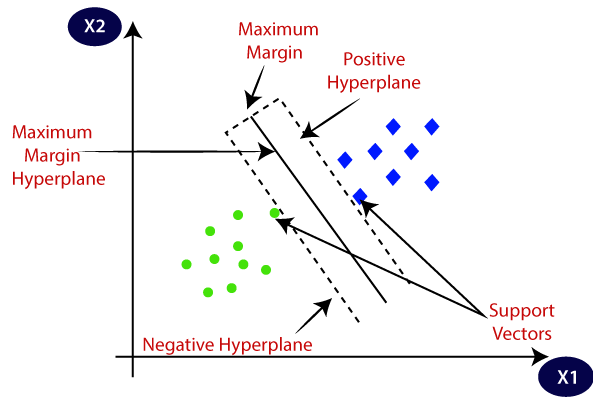
\includegraphics[width=.5\textwidth]{ej_svm}
  \caption{Ejemplo de SVM lineal.}
  \label{fig:ej-svm}
\end{figure}

Además se puede incluir una transformación no lineal en los datos para intentar conseguir una mejor separación en otros espacios, mediante la denominada función \emph{kernel}. Las más usadas son las siguientes, siendo $\gamma$ un hiperparámetro:

  \begin{enumerate}
    \item Polinómica de grado $d$ y radio $r$: $(\gamma<x, x'> + r)^d$.
    \item Base radial (\emph{Radial Basis Function}, RBF): $\exp(-\gamma||x - x'||^2_2)$.
    \item Sigmoide de radio $r$: $\tanh(\gamma<x, x'> + r)$.
  \end{enumerate}

Para nuestro modelo fijamos el parámetro de regularización $C$ a 1 (cuanto más vale, menos fallos permite), usando como función \emph{kernel} RBF y dejamos que $\gamma$ tome un valor heurístico a $1 / (M * Var(X))$ siendo $M$ el número de características y $X$ los datos.

\subsection{Árboles de decisión}

Los árboles de decisión son un modelo muy simple que se puede entender como un conjunto de \textbf{reglas} asociadas a las características (\autoref{fig:ej-dt}), o como una serie de hiperplanos paralelos a los ejes que particionan el espacio. Estas reglas nos permiten \textbf{entender} porqué el árbol llega a la predicción, cosa que no suele suceder en la mayoría de modelos.

\begin{figure}[htbp]
  \centering
  %\hspace*{-2.5cm}
  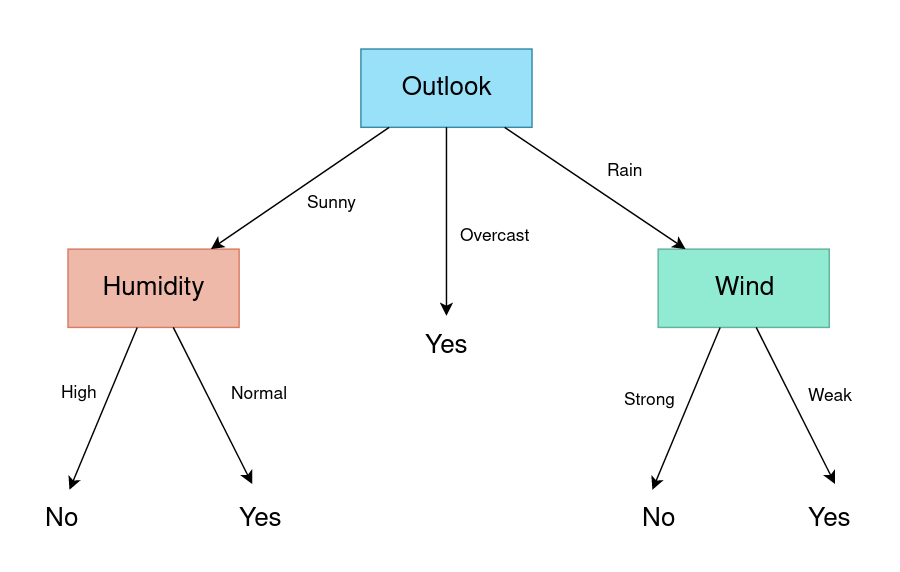
\includegraphics[width=.5\textwidth]{ej_dt}
  \caption{Árbol de decisión con reglas para si debería jugar al tenis.}
  \label{fig:ej-dt}
\end{figure}

En general el gran problema que presentan es el alto \textbf{sobreajuste} que tienen: a costa de tener un error/sesgo casi nulo se tiene demasiada varianza. Por ejemplo, para dos muestras de datos un poco distintas pueden dar lugar a dos árboles completamente distintos.

Usamos unos cuantos subtipos/implementaciones usualmente utilizados:

\begin{itemize}
  \item \textbf{CART}: Classification and Regression Trees \cite{breiman1984classification} implementado en \emph{Python} en la librería \emph{scikit-learn} \cite{scikit2020dt}. Fijamos la profundidad máxima a 20 para evitar sobreajuste.
  \item \textbf{C4.5}: \cite{quinlan2014c4} implementado en \emph{R} en el paquete \emph{partykit} \cite{hornik2020c45}.
  \item \textbf{C5.0}: mejora de C4.5 \cite{quinlan2019c50} implementado en \emph{R} en el paquete \emph{C50} \cite{kuhn2020c50}. Se añade un modelo sin \emph{boosting} y otro con 10 árboles.
  \item \textbf{RPart}: Recursive partitioning for classification trees \cite{breiman1984classification} implementado en \emph{R} en el paquete \emph{rpart} \cite{atkinson2019rpart}.
  \item \textbf{CTree}: Conditional inference tree \cite{hothorn2006unbiased, hothorn2015ctree} implementado en \emph{R} en el paquete \emph{ctree} \cite{hothorn2020ctree}.
\end{itemize}

Excepto CART, para el resto se ha usado la librería \emph{rpy2} \cite{gautier2020rpy2} para usar en \emph{Python} las clases en \emph{R}.

\subsection{Random Forest}

Random Forest \cite{ho1995random, breiman2001random} con implementacion en \emph{Python} de la librería \emph{scikit-learn} \cite{scikit2020rf}. Un modelo no lineal que construye una \textbf{agrupación} (\emph{ensemble}) de árboles de decisión mediante la técnica de \emph{bootsrap}/\emph{bagging}. La idea detrás de este método es \textbf{evitar} el sobreajuste ocasionado por la alta varianza que tiene un solo árbol de decisión, utilizando un gran cantidad de ellos y además entrenándolos cada uno con sola muestra aleatoria con reemplazamiento (\autoref{fig:ej-rf} \cite{orellana2018rf}).

\begin{figure}[htbp]
  \centering
  %\hspace*{-2.5cm}
  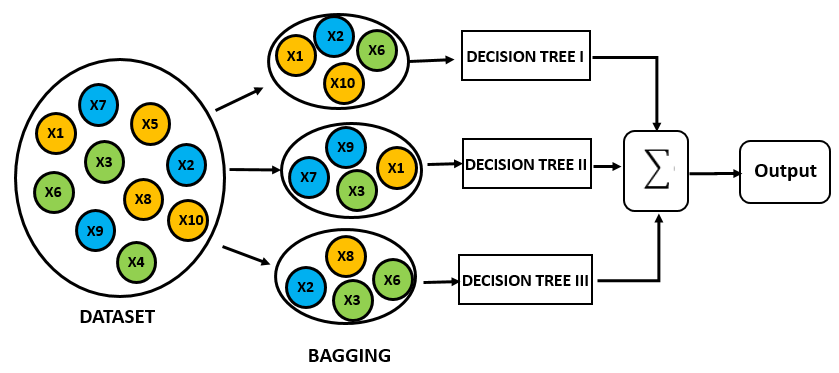
\includegraphics[width=.6\textwidth]{ej_rf}
  \caption{Construcción de Random Forest.}
  \label{fig:ej-rf}
\end{figure}

Como en los árboles, el espacio se particiona por hiperplanos paralelos a los ejes, considerando que ahora se toma el voto mayoritario de la agrupación de todos. Sin embargo se pierde la interpretabilidad clara que pudiera tener un solo árbol, si bien podemos intentar observar las características más importantes según la cantidad de veces que aparecen en los árboles.

Usando una regla heurística se fija el número de características de cada árbol a $\sqrt{M}$ siendo $M$ el número de características del \emph{dataset} y usamos el criterio de la impureza Gini \cite{rokach2005top} para escoger las características que dividen al árbol.

Escogemos para el modelo 200 árboles con una profundidad máxima de 20, que según el \emph{dataset} podrá ser poco o mucho pero en principio lo ponemos así para evitar en la medida de lo posible un sobreajuste constante.

\subsection{$k$-NN}

$k$-Nearest Neighbors ($k$-NN) \cite{cover1967nearest} usando como base la implementación en \emph{Python} de la librería \emph{scikit-learn} \cite{scikit2020knn}. Es un modelo no lineal simple que cambia el enfoque de los modelos anteriores. El entrenamiento consiste únicamente en \textbf{copiar} los datos, de manera que para clasificar un punto considera los $k$ vecinos (datos) \textbf{más cercanos} de los que fueron guardados, en función de la métrica que se le haya indicado. Por tanto lo que realiza el modelo es una partición del espacio cuya forma estará determinada por la distribución de los datos y el $k$ elegido; un ejemplo lo tenemos en \autoref{fig:ej-knn} \cite{sanjay2018knn}.

\begin{figure}[htbp]
  \centering
  %\hspace*{-2.5cm}
  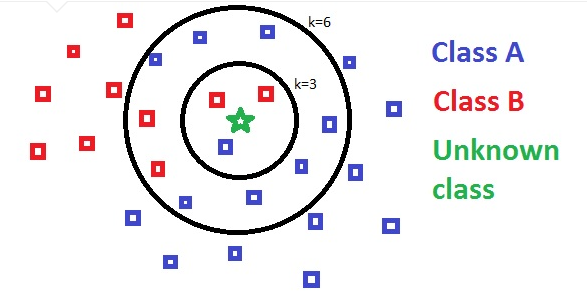
\includegraphics[width=.6\textwidth]{ej_knn}
  \caption{Ejemplo de $k$-NN. Con $k=3$ se toma la clase B, con $k=6$ la A.}
  \label{fig:ej-knn}
\end{figure}

Para nuestro modelo consideramos la métrica usual euclídea $||\cdot||_2$ y usamos la regla heurística que recomienda usar $k \approx \sqrt{N}$ siendo $N$ el número de series del \emph{dataset} de entrenamiento.

Como estamos en el contexto de las series temporales, se ha decidido añadir otro modelo $k$-NN pero en vez de usar la métrica euclidea usamos la \emph{semi}-métrica \emph{Dynamic Time Warping} ($DTW$) \cite{berndt1994using}. Esta \emph{semi-}métrica \cite{jain2018semi} mide la distancia con el \textbf{alineamiento óptimo} entre dos series temporales, de manera que es muy útil para medir series que exhiben ciertos patrones pero que tienen \textbf{pequeñas variaciones} (por ejemplo, una pequeña amplitud o desplazamiento) entre sí. Si suponemos que las series con misma etiqueta siguen una cierta forma bajo esta distancia deberían obtener valores muy bajos, si lo unimos con el algoritmo $k$-NN tenemos un modelo que puede funcionar bastante bien.

Ejemplificamos visualmente lo que calcula $DTW$ comparando con la métrica euclídea en \autoref{fig:ej-dtw} \cite{volny2012employing}; observamos que para cada punto se busca la mejor coincidencia con la otra serie, consiguiendo una buena correspondencia entre series parecidas.

\begin{figure}[htbp]
  \centering
  %\hspace*{-2.5cm}
  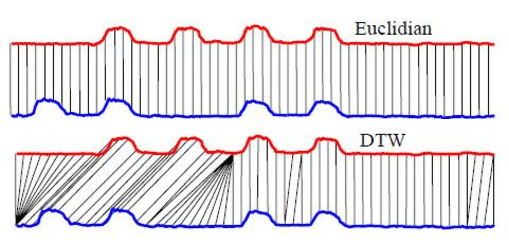
\includegraphics[width=0.6\textwidth]{ej_dtw}
  \caption{Funcionamiento de $DTW$ frente $||\cdot||_2$.}
  \label{fig:ej-dtw}
\end{figure}

Sin embargo, $DTW$ es muy \textbf{costoso} de usar, puesto que para cada punto de la serie se calcula una distancia ($||\cdot||_1$ o $||\cdot||_2$) con el resto de puntos de la otra serie, y si tenemos en cuenta que en $k$-NN se calculan las distancias de cada serie que se quiera etiquetar con todas las series de entrenamiento el tiempo empleado en cómputos se dispara. Por ello para nuestro modelo usaremos una implementación eficiente en R \cite{leodolter2020dtw} junto al uso de una ventana de tamaño 5 (solo se buscan las coincidencias en un entorno de radio 5). Finalmente fijamos $k = 3$ ya que esperamos una mejor agrupación con $DTW$ (podríamos haber cogido $k=1$ pero si hacemos esto provocaríamos que $acc_{train} = 1$, sobreajustando demasiado) y evitamos aumentar aún más los cálculos.

El modelo $k-NN$ euclideo para tomar el $k$ automático se ha implementado en \emph{Python} y para $k$-NN + $DTW$ se ha usado otra vez la librería \emph{rpy2} para usar el paquete de \emph{R} en \emph{Python}.

\section{Experimentación previa}

Antes de hacer un trabajo de experimentación extenso se hicieron varias pruebas para determinar la eficacia previa del $PV$, no se detalla en concreto ya que fueron pequeños casos (unos cuantos \emph{datasets} y clasificadores) de los experimentos grandes que comentaremos en \autoref{ch:pv-experimentacion} para poder corroborar rápidamente los resultados en \cite{zhang2019perturbation} y comprobar la viabilidad de los experimentos. Se pudieron notar los siguientes aspectos:

\begin{enumerate}
  \item La \textbf{forma} de los puntos: como se indicaba en \cite{zhang2019perturbation}, la puntos $\{r_i, acc_i\}$ se alinean con una recta con pendiente no positiva generalmente, los puntos a veces pueden estar un poco por encima/debajo de ella pero se ve claramente la tendencia de recta.

  \item El \textbf{tamaño} del \emph{dataset}: un \emph{dataset} muy pequeño (depende de lo complicada que sea la distribución original) puede dar lugar a que el $PV$ sea muy inestable entre ejecuciones debido a la aleatoriedad de escoger y cambiar etiquetas. No es especialmente preocupante puesto que para que los modelos aprendan correctamente se necesita una cantidad importante de datos.

  \item El \textbf{intervalo} donde tomar los $r_i$ (errores): la propuesta original de \cite{zhang2019perturbation} indicaba el intervalo $[0, 0.5]$ pero se obtuvieron resultados que indicaban que a partir de $0.4$ las alteraciones eran demasiado fuertes. Nuestras observaciones concuerdan con la nueva versión de \cite{zhang2019perturbation}, que restringieron a $[0, 0.3]$.

  \item Valores \textbf{válidos} de $n$ (número de \emph{datasets} perturbados): \cite{zhang2019perturbation} indica usar solamente 3, aunque es posible tomar cualquier valor mayor que este. Cuantos más puntos más robusto será el valor $PV$ aunque computacionalmente será más costoso, por lo que un valor de 5 es más que razonable para obtener resultados buenos.

  \item \textbf{Rango} de valores del $PV$: como reflejan en \cite{zhang2019perturbation} la mayoría de valores del $PV$ obtenidos se encuentran en el intervalo $[0, 1]$ si bien se obtienen a veces valores por encima. Para los valores en $[1, 2]$, en \cite{zhang2019perturbation} se propone corregirlos al $[0, 1]$ penalizándolos con la   transformación \eqref{eq:pv-penalizacion}. En nuestro caso dejaremos los datos originales sin transformar, para notar explícitamente que se han obtenido estos valores por encima de los usuales.

  \begin{equation}
    PV_{corregido} = 1 - |PV - 1|.
    \label{eq:pv-penalizacion}
  \end{equation}

  \item \textbf{Interpretabilidad} del $PV$: el $PV$ nos indica en líneas generales si el modelo ha entendido correctamente el patrón subyacente en los datos. Observamos que conforme \textbf{aumenta} $PV$, el valor de las métricas $acc_{train}$ y $acc_{test}$ también lo hace y la tendencia del sobreajuste disminuye.

  \item \textbf{Resultados} del $PV$: observamos que modelos que obtienen un $PV \approx 0$ suelen tener un $acc_{train}$ bastante alto mientras que en $acc_{CV}$ y $acc_{test}$ bajan bastante, haciéndose evidente el sobreajuste que existe. Además, un modelo puede tener mejor $PV$ que otro pero no tiene por qué mantenerse el orden con $acc_{test}$; lo que sí observamos es que conforme aumenta $PV$, la tasa de $acc_{train}$ y $acc_{test}$ aumentan y el sobreajuste disminuye.

  \item \textbf{Cambio en las perturbaciones}: se intentó probar a perturbar los datos en sí en vez de las etiquetas (para poder trasladar el $PV$ a problemas con métricas continuas o problemas no supervisados) con distintas pruebas, por ejemplo ruido gaussiano; pero no tuvieron el efecto deseado y al no tener unos resultados muy claros se decidió descartar esta línea.

\end{enumerate}

Como los resultados de \cite{zhang2019perturbation} parecían corresponder con estos preliminares dimos el visto bueno para pasar a la experimentación extendida para comprobar de una manera más extendida y analizar detalladamente la eficacia y los resultados del $PV$.

\section{Elección del mejor modelo}

\subsection{Descripción}

\subsubsection{Objetivos}

En este experimento evaluamos la nueva heurística $PV$ frente a las medidas clásicas de validación $acc_{CV}$ y $acc_{test}$. De \cite{zhang2019perturbation} y la experimentación previa sabemos que aunque un modelo obtenga un mejor valor de $PV$ frente a otro (sobre todo cuando los $PV$ rondan valores muy bajos) esto no implicará con una seguridad absoluta que el $acc_{test}$ sea mejor también, sobretodo si el rango del $PV$ es bajo (en un entorno cercano al 0).

Por tanto lo que esperamos en este experimento es:

\begin{enumerate}
  \item Que un $PV$ alto indique que el modelo sea \textbf{bueno}: esperamos que un modelo sea bueno si la función aprendida se \textbf{corresponde con la función de la distribución} de los datos. Sin embargo como desconocemos esta función no podemos compararlas para comprobarlo directamente pensamos que si el modelo ha aprendido la función correcta deberá obtener una \textbf{buena tasa de acierto} en \textbf{cualquier conjunto} de datos, es decir deberá obtener un valor en ambas métricas $acc_{train}$ y $acc_{test}$ y ser muy iguales, ya que no debería haber \textbf{sobreajuste}.

  \item Si $PV \approx 0$ el modelo \textbf{sobreajustará}: si el $PV \approx 0$ entendemos que la complejidad del modelo es superior a la necesaria o bien no ha conseguido entender nada de la función de etiquetado. En cualquier caso esperamos que en otra muestra distinta el modelo lo haga mucho peor, notando una tasa de $acc_{test}$ peor y probablemente con una gran diferencia con $acc_{train}$ si el modelo se ha pasado con la complejidad.
\end{enumerate}

\subsubsection{Datasets}

Utilizamos la base de datos "\emph{UEA \& UCR Time Series Classification}" \cite{bagnall2020ts} que reune 158 \emph{dataset} de series temporales estandarizadas para problemas de clasificación. Cogeremos los 114 \emph{datasets} de series temporales \textbf{unidimensionales} para evitar altos tiempos en entrenamiento, mezclamos la partición ya hecha en \emph{train}/\emph{test} ya que muchos \emph{datasets} \emph{train} tienen \textbf{muy} pocas series y hay un gran desequilibrio, y volvemos a partir pero con un 80/20\%. Finalmente nos quedaremos con los que el \emph{dataset} \emph{train} cumpla las siguientes condiciones:

\begin{enumerate}
  \item Tiene al menos \textbf{100 series}: aunque puede depender de la distribución, en general necesitamos muchos datos para que los modelos aprendan. Además un número tan pequeño de series puede ocasionar una gran inestabilidad a la hora de obtener el $PV$.
  \item Tiene al menos \textbf{5 series por clase}: si no se tiene al menos 5 elementos por clase (se podría poner un umbral mayor incluso) como al hacer el $PV$ alteramos las etiquetas el error que introducimos sería demasiado fuerte.
  \item La clase mayoritaria no tiene una \textbf{proporción mayor al 70\%}: usamos la métrica $acc$ por lo que evitamos \emph{datasets} con un gran desequilibrio entre número de instancias por clase.
\end{enumerate}

Además de considerar los \emph{datasets} originales en medida temporal (TS), también tomaremos su versión en medidas de complejidad (CMFTS). La lista final de los 95 \emph{datasets} se encuentra detallada en \autoref{table:pv-datasets1} y \autoref{table:pv-datasets2}.

\begin{table}[htbp]
\centering
\hspace*{-1cm}
%\hspace*{-2.2cm}
\begin{tabular}{||l c c c c c||}
 \hline
 Nombre & Tamaño Train & Tamaño Test & Nº clases & Longitud TS & Longitud CMFTS \\ [0.5ex]
 \hline\hline
 ACSF1 & 160 & 40 & 10 & 1460 & 38 \\
 Adiac & 624 & 157 & 37 & 176 & 38 \\
 ArrowHead & 168 & 43 & 3 & 251 & 38 \\
 BME & 144 & 36 & 3 & 128 & 38 \\
 CBF & 744 & 186 & 3 & 128 & 38 \\
 ChlorineConcentration & 3445 & 862 & 3 & 166 & 37 \\
 CinCECGTorso & 1136 & 284 & 4 & 1639 & 38 \\
 Computers & 400 & 100 & 2 & 720 & 38 \\
 CricketX & 624 & 156 & 12 & 300 & 38 \\
 CricketY & 624 & 156 & 12 & 300 & 38 \\
 CricketZ & 624 & 156 & 12 & 300 & 38 \\
 Crop & 19200 & 4800 & 24 & 46 & 36 \\
 DiatomSizeReduction & 257 & 65 & 4 & 345 & 36 \\
 DistalPhalanxOutlineAgeGroup & 431 & 108 & 3 & 80 & 36 \\
 DistalPhalanxOutlineCorrect & 700 & 176 & 2 & 80 & 36 \\
 DistalPhalanxTW & 431 & 108 & 6 & 80 & 36 \\
 ECG200 & 160 & 40 & 2 & 96 & 36 \\
 ECG5000 & 4000 & 1000 & 5 & 140 & 38 \\
 ECGFiveDays & 707 & 177 & 2 & 136 & 38 \\
 ElectricDevices & 13309 & 3328 & 7 & 96 & 36 \\
 EOGHorizontalSignal & 579 & 145 & 12 & 1250 & 38 \\
 EOGVerticalSignal & 579 & 145 & 12 & 1250 & 38 \\
 EthanolLevel & 803 & 201 & 4 & 1751 & 37 \\
 FaceAll & 1800 & 450 & 14 & 131 & 38 \\
 FacesUCR & 1800 & 450 & 14 & 131 & 38 \\
 FiftyWords & 724 & 181 & 50 & 270 & 38 \\
 Fish & 280 & 70 & 7 & 463 & 37 \\
 FordA & 3936 & 985 & 2 & 500 & 38 \\
 FordB & 3556 & 890 & 2 & 500 & 38 \\
 FreezerRegularTrain & 2400 & 600 & 2 & 301 & 38 \\
 FreezerSmallTrain & 2302 & 576 & 2 & 301 & 38 \\
 Fungi & 163 & 41 & 18 & 201 & 38 \\
 GunPoint & 160 & 40 & 2 & 150 & 38 \\
 GunPointAgeSpan & 360 & 91 & 2 & 150 & 38 \\
 GunPointMaleVersusFemale & 360 & 91 & 2 & 150 & 38 \\
 GunPointOldVersusYoung & 360 & 91 & 2 & 150 & 38 \\
 Ham & 171 & 43 & 2 & 431 & 38 \\
 HandOutlines & 1096 & 274 & 2 & 2709 & 37 \\
 Haptics & 370 & 93 & 5 & 1092 & 38 \\
 Herring & 102 & 26 & 2 & 512 & 37 \\
 HouseTwenty & 127 & 32 & 2 & 2000 & 38 \\
 InlineSkate & 520 & 130 & 7 & 1882 & 37 \\
 InsectEPGRegularTrain & 248 & 63 & 3 & 601 & 38 \\
 InsectEPGSmallTrain & 212 & 54 & 3 & 601 & 38 \\
 InsectWingbeatSound & 1760 & 440 & 11 & 256 & 38 \\
 ItalyPowerDemand & 876 & 220 & 2 & 24 & 36 \\
 LargeKitchenAppliances & 600 & 150 & 3 & 720 & 38 \\
 Lightning7 & 114 & 29 & 7 & 319 & 38 \\ [1ex]
 \hline
\end{tabular}
\caption{Datasets del experimento.}
\label{table:pv-datasets1}
\end{table}

\begin{table}[htbp]
\centering
\hspace*{-2cm}
%\hspace*{-0.9cm}
\begin{tabular}{||l c c c c c||}
 \hline
 Nombre & Tamaño Train & Tamaño Test & Nº clases & Longitud TS & Longitud CMFTS \\ [0.5ex]
 \hline\hline
 Mallat & 1920 & 480 & 8 & 1024 & 38 \\
 MedicalImages & 912 & 229 & 10 & 99 & 38 \\
 MelbournePedestrian & 2920 & 730 & 10 & 24 & 36 \\
 MiddlePhalanxOutlineAgeGroup & 443 & 111 & 3 & 80 & 36 \\
 MiddlePhalanxOutlineCorrect & 712 & 179 & 2 & 80 & 36 \\
 MiddlePhalanxTW & 442 & 111 & 6 & 80 & 36 \\
 MixedShapesRegularTrain & 2340 & 585 & 5 & 1024 & 38 \\
 MixedShapesSmallTrain & 2020 & 505 & 5 & 1024 & 38 \\
 MoteStrain & 1017 & 255 & 2 & 84 & 36 \\
 NonInvasiveFetalECGThorax1 & 3012 & 753 & 42 & 750 & 38 \\
 NonInvasiveFetalECGThorax2 & 3012 & 753 & 42 & 750 & 38 \\
 OSULeaf & 353 & 89 & 6 & 427 & 38 \\
 PhalangesOutlinesCorrect & 2126 & 532 & 2 & 80 & 36 \\
 Plane & 168 & 42 & 7 & 144 & 38 \\
 PowerCons & 288 & 72 & 2 & 144 & 38 \\
 ProximalPhalanxOutlineAgeGroup & 484 & 121 & 3 & 80 & 35 \\
 ProximalPhalanxOutlineCorrect & 712 & 179 & 2 & 80 & 35 \\
 ProximalPhalanxTW & 484 & 121 & 6 & 80 & 35 \\
 RefrigerationDevices & 600 & 150 & 3 & 720 & 38 \\
 ScreenType & 600 & 150 & 3 & 720 & 38 \\
 SemgHandGenderCh2 & 720 & 180 & 2 & 1500 & 38 \\
 SemgHandMovementCh2 & 720 & 180 & 6 & 1500 & 38 \\
 SemgHandSubjectCh2 & 720 & 180 & 5 & 1500 & 38 \\
 ShapeletSim & 160 & 40 & 2 & 500 & 38 \\
 ShapesAll & 960 & 240 & 60 & 512 & 38 \\
 SmallKitchenAppliances & 600 & 150 & 3 & 720 & 38 \\
 SmoothSubspace & 240 & 60 & 3 & 15 & 30 \\
 SonyAIBORobotSurface1 & 496 & 125 & 2 & 70 & 36 \\
 SonyAIBORobotSurface2 & 784 & 196 & 2 & 65 & 36 \\
 StarLightCurves & 7388 & 1848 & 3 & 1024 & 38 \\
 Strawberry & 786 & 197 & 2 & 235 & 38 \\
 SwedishLeaf & 900 & 225 & 15 & 128 & 38 \\
 Symbols & 816 & 204 & 6 & 398 & 38 \\
 SyntheticControl & 480 & 120 & 6 & 60 & 36 \\
 ToeSegmentation1 & 214 & 54 & 2 & 277 & 38 \\
 Trace & 160 & 40 & 4 & 275 & 38 \\
 TwoLeadECG & 929 & 233 & 2 & 82 & 36 \\
 TwoPatterns & 4000 & 1000 & 4 & 128 & 38 \\
 UMD & 144 & 36 & 3 & 150 & 38 \\
 UWaveGestureLibraryAll & 3582 & 896 & 8 & 945 & 38 \\
 UWaveGestureLibraryX & 3582 & 896 & 8 & 315 & 38 \\
 UWaveGestureLibraryY & 3582 & 896 & 8 & 315 & 38 \\
 UWaveGestureLibraryZ & 3582 & 896 & 8 & 315 & 38 \\
 WordSynonyms & 724 & 181 & 25 & 270 & 38 \\
 Worms & 206 & 52 & 5 & 900 & 38 \\
 WormsTwoClass & 206 & 52 & 2 & 900 & 38 \\
 Yoga & 2640 & 660 & 2 & 426 & 38 \\ [1ex]
 \hline
\end{tabular}
\caption{Datasets del experimento (continuación).}
\label{table:pv-datasets2}
\end{table}

\subsubsection{Clasificadores}

Ya comentábamos previamente los modelos utilizados, así que los listamos simplemente ahora:

\begin{itemize}
  \item \textbf{LSTM}: Con la arquitectura ya indicada, se entrena como máximo 300 épocas con tamaño de \emph{batch} a 128 y un 10\% de validación, parando si no hay una mejora de al menos de 0.1 en $acc_{val}$ en 50 épocas y quedándose con la configuración que mejor $acc_{val}$ haya tenido.
  \item \textbf{SVM}: $C = 1$, función de \emph{kernel} RBF y $\gamma = 1 / (M * Var(X))$ ($M$ longitud series y $Var(X)$ varianza de las series).
  \item \textbf{CART}: profundidad máxima de 20.
  \item \textbf{C4.5}.
  \item \textbf{C5.0}.
  \item \textbf{C5.0 + boosting}: \emph{boosting} con 10 árboles.
  \item \textbf{RPart}.
  \item \textbf{CPart}.
  \item \textbf{Random Forest}: 200 árboles con profundidad máxima de 20.
  \item \textbf{$k$-NN euclideo}: $k = \sqrt{N}$ siendo $N$ el número de series de entrenamiento.
  \item \textbf{$k$-NN + DTW}: $k = 3$ y tamaño de ventana a 5.
\end{itemize}

Notamos que estos modelos no estarán adecuados con la mejor configuración de hiperparámetros para cada \emph{dataset} pero se puede seguir haciendo la comparación mediante las métricas.

\subsubsection{Métricas}

Las métricas a medir son:

\begin{itemize}
  \item $PV$: la nueva heurística a medir, tomando $n = 5$, $r_1 = 0.1$ y $r_n = 0.3$.
  \item $acc_{train}$: acierto en el conjunto de entrenamiento.
  \item $acc_{CV}$: acierto por validación cruzada con 5 particiones en el \emph{dataset} de entrenamiento.
  \item $acc_{test}$: acierto en el conjunto test.
\end{itemize}

Guardaremos también los resultados de los $acc_i$ obtenidos al calcular el $PV$.

\subsection{Resultados}

Hemos guardado dos tipos de resultados, disponibles en el \href{https://github.com/MiguelLentisco/tfg}{repositorio del proyecto}:

\begin{itemize}
  \item Los valores de cada métrica para cada clasificador en un archivo de tipo \emph{csv} (NombreDataset.csv). Un ejemplo formateado a tabla sería \autoref{table:ejemplo-tabla}.
  \item Una gráfica mostrando los puntos ${(r_i, acc_i)}$ obtenidos para cada clasificador para calcular el PV, junto con la regresión lineal obtenida. Un ejemplo lo tenemos en \autoref{fig:res-imagen}.
\end{itemize}

\begin{table}[htbp]
\centering
%\hspace*{-2cm}
\hspace*{-0.9cm}
\begin{tabular}{||l | c c c c c c c c c||}
 \hline
 Classifier & $PV$ & $acc_{train}$ & $acc_{CV}$ & $acc_{test}$ & $acc_1$ & $acc_2$ & $acc_3$ & $acc_4$ & $acc_5$ \\ [0.5ex]
 \hline\hline
 RBF-SVM & 0.1763 & 0.1378 & 0.1385 & 0.1592 & 0.1298 & 0.1234 & 0.1202 & 0.1154 & 0.0897 \\
 Random Forest &0.0 & 1.0 & 0.6856 & 0.7389 & 1.0 & 1.0 & 1.0 & 1.0 & 1.0 \\
 CART & 0.0833 & 0.9968 & 0.5012 & 0.5223 & 1.0 & 1.0 & 0.9936 & 0.9872 & 0.9856 \\
 C4.5 & 0.4647 & 0.9263 & 0.5481 & 0.5987 & 0.859 & 0.867 & 0.8189 & 0.8045 & 0.774 \\
 C5.0 & 0.4615 & 0.9263 & 0.5562 & 0.6306 & 0.8622 & 0.851 & 0.8349 & 0.8029 & 0.7708 \\
 C5.0-Boosting & 0.0833 & 1.0 & 0.6443 & 0.7261 & 0.9952 & 0.9952 & 0.9952 & 0.9856 & 0.9792 \\
 CTree & 0.9423 & 0.5577 & 0.3942 & 0.465 & 0.4311 & 0.4199 & 0.3814 & 0.3141 & 0.2484 \\
 RPart & 0.9327 & 0.6635 & 0.4791 & 0.5096 & 0.6154 & 0.5545 & 0.5401 & 0.4792 & 0.4199 \\
 kNN & 0.5481 & 0.5192 & 0.4023 & 0.4586 & 0.4551 & 0.4535 & 0.4183 & 0.3814 & 0.3542 \\
 3NN+DTW & 0.0288 & 0.8846 & 0.4616 & 0.5159 & 0.8798 & 0.8718 & 0.8766 & 0.8606 & 0.8926 \\
 LSTM & 1.5513 & 0.391 & 0.4343 & 0.3376 & 0.4503 & 0.0417 & 0.2292 & 0.0417 & 0.0625 \\ [1ex]
 \hline
\end{tabular}
\caption{Resultados de Adiac.csv versión TS.}
\label{table:ejemplo-tabla}
\end{table}

\begin{figure}[htbp]
  \centering
  \hspace*{-1cm}
  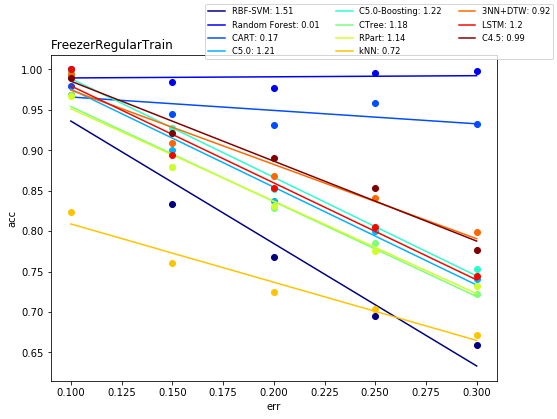
\includegraphics[width=0.8\textwidth]{res-imagen}
  \caption{Resultados $acc$ y recta de regresión al calcular $PV$ en FreezerRegularTrain versión TS.}
  \label{fig:res-imagen}
\end{figure}

Unimos todos los datos obtenidos para poder visualizar la relación entre la heurística $PV$ y las métricas existentes, a los que añadimos unas rectas de regresión para mostrar la tendencia de los datos, aunque en un caso se ha tenido que usar una parábola de regresión (\autoref{fig:res-pv}). Además se ha añadido la distribución en un histograma de los valores del $PV$ (\autoref{fig:dist-pv}).

\begin{figure}[htbp]
  \centering
  \hspace*{-1cm}
  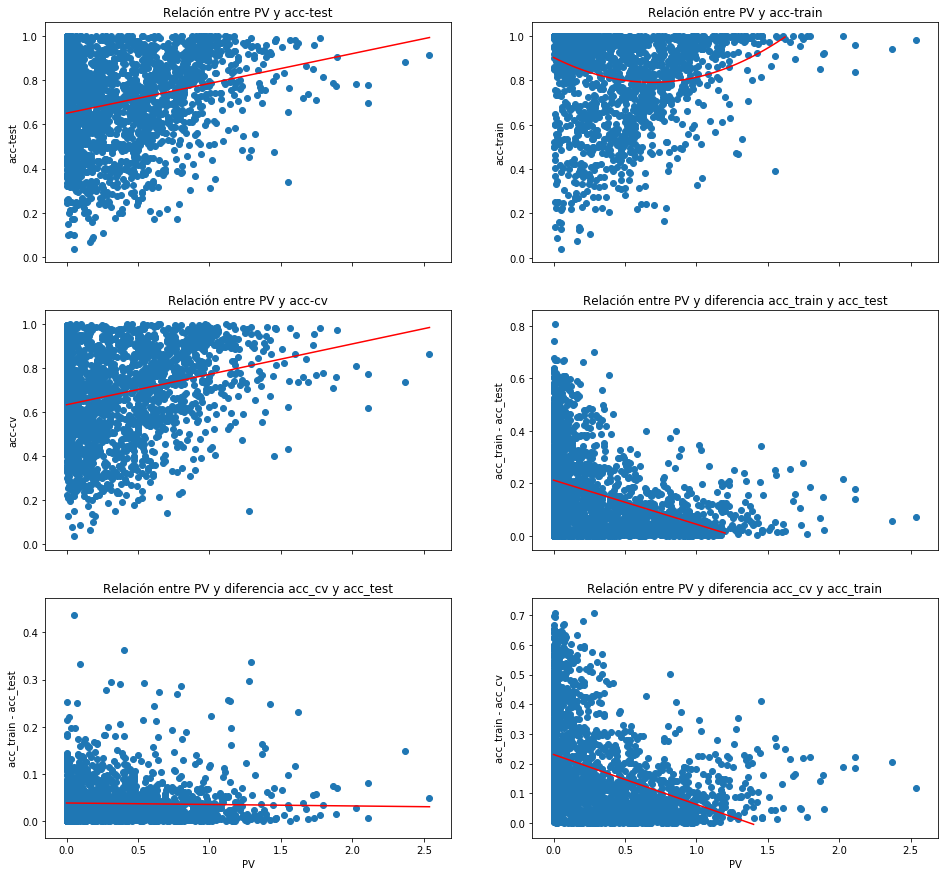
\includegraphics[width=1.2\textwidth]{res_pv}
  \caption{Relaciones entre $PV$ y otras métricas.}
  \label{fig:res-pv}
\end{figure}

\begin{figure}[htbp]
  \centering
  %\hspace*{-1cm}
  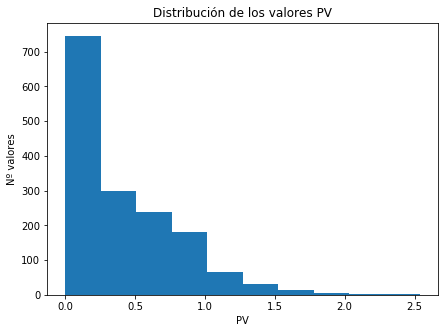
\includegraphics[width=0.7\textwidth]{dist_pv}
  \caption{Distribución de valores del $PV$.}
  \label{fig:dist-pv}
\end{figure}

Finalmente hemos recogido en una tabla ciertos valores interesantes de cada modelo para estudiar sus comportamientos individuales: los valores máximos, mínimos, media, desviación típica y número de valores por encima de 1 de $PV$; la media de $acc_{train}$ y $acc_{test}$ y finalmente la media y desviación típica de los errores cuadráticos medios de la regresión lineal obtenida en el cálculo del $PV$ (\autoref{table:datos-modelos})

\begin{table}[htbp]
\centering
%\hspace*{-2cm}
\hspace*{-0.9cm}
\begin{tabular}{||l | c c c c c c c c c||}
 \hline
 Classifier & $\min PV$ & $\max PV$ & $\overline{PV}$ & $\sigma_{PV}$ & $|PV > 1|$ & $\overline{acc_{train}}$ & $\overline{acc_{test}}$ & $\overline{MSE}$ & $\sigma_{MSE}$ \\ [0.5ex]
 \hline\hline
 RBF-SVM & 0.000 & 1.111 & 0.511 & 0.302 & 6 & 69.866\% & 65.329\% & 0.0001 & 0.0003 \\
 Random Forest & 0.000 & 0.285 & 0.017 & 0.048 & 0 & 99.955\% & 79.916\% & 0.0000 & 0.0000 \\
 CART & 0.000 & 0.858 & 0.060 & 0.110 & 0 & 99.608\% & 70.883\% & 0.0001 & 0.0002 \\
 C4.5 & 0.000 & 2.112 & 0.440 & 0.435 & 26 & 94.114\% & 71.776\% & 0.0012 & 0.0032 \\
 C5.0 & 0.006 & 1.747 & 0.392 & 0.369 & 18 & 93.478\% & 72.474\% & 0.0007 & 0.0014 \\
 C5.0-Boosting & 0.000 & 2.025 & 0.363 & 0.512 & 33 & 98.033\% & 77.784\% & 0.0008 & 0.0022 \\
 CTree & 0.000 & 2.366 & 0.731 & 0.342 & 28 & 72.754\% & 67.755\% & 0.0006 & 0.0013 \\
 RPart & 0.000 & 0.995 & 0.518 & 0.248 & 0 & 77.188\% & 67.841\% & 0.0003 & 0.0004 \\
 kNN & 0.008 & 0.977 & 0.519 & 0.253 & 0 & 69.065\% & 66.173\% & 0.0002 & 0.0004 \\
 3NN+DTW & 0.000 & 0.763 & 0.246 & 0.186 & 0 & 90.052\% & 72.121\% & 0.0002 & 0.0003 \\
 LSTM & 0.007 & 2.540 & 0.593 & 0.472 & 37 & 67.746\% & 62.959\% & 0.0050 & 0.0059 \\ [1ex]
 \hline
\end{tabular}
\caption{Diferentes resultados de cada modelo.}
\label{table:datos-modelos}
\end{table}

\subsection{Análisis}

Observando \autoref{fig:res-pv} podemos comprobar que las hipótesis que queríamos comprobar estaban en lo correcto: cuando $PV$ aumenta, la tendencia de $acc_{test}$ y $acc_{train}$ es creciente indicando que los modelos son \textbf{buenos} en cuanto a \textbf{mejor ajuste} y menor \textbf{sobreajuste}; notándose además que cuando $PV \approx 0$ observamos un gran cúmulo de valores de $acc_{train} \approx 1$ mientras que $acc_{test}$ toma valores en toda la franja $[0,1]$ manifestándose en el \textbf{fuerte sobreajuste} que existe en ciertos modelos (razón por la que hemos usado una parábola de regresión).

Además entre $PV$ y $acc_{CV}$, como $acc_{CV}$ es un estimador de $acc_{test}$, se tiene una relación muy idéntica entre $PV$ y $acc_{test}$. También es notable el hecho de que conforme aumenta $PV$ la diferencia entre $acc_{CV}$ y $acc_{test}$ disminuya ligeramente, indicando que $acc_{CV}$ se vuelve mejor estimador (menor varianza) conforme más vale sea $PV$.

Por otro lado, queda claro que $PV$ no nos marca el modelo que mayor $acc_{test}$ tenga, observamos que hay valores altos de $acc_{test}$ a pesar de que el $PV$ sea bajo; incluso con valores más grandes de $PV$ no se nos puede asegurar nada, pero probablemente tengan unos muy buenos resultados.

De \autoref{fig:dist-pv} notamos que la mayoría de valores se concentran en el intervalo esperado $[0, 1]$ con una pequeña franja en $[1, 1.5]$ que era posible también. Únicamente se han detectado una pequeña cantidad de puntos (una veintena) en $[1.5, 2]$, y únicamente 5 puntos en $[2, 2.6]$, que aunque en principio son valores atípicos respecto de la distribución del $PV$ los estudiaremos más adelante para intentar averiguar las causas de estos valores.

En \autoref{table:datos-modelos} tenemos distintos datos que resaltan: lo más notable es los resultados de los modelos C4.5, C5.0 (sin y con \emph{boosting}), CTree y LSTM que obtienen unos valores $\max PV$ bastante por encima de 1, que se une con una mayor dispersión $\sigma_{PV}$, una cantidad alta de valores atípicos $|PV > 1|$ y unos mayores errores de ajuste en las rectas de regresión para calcular el $PV$ tanto en la media $\overline{MSE}$ como en la dispersión $\sigma_{MSE}$.

Todos estos indicadores nos están diciendo que para estos modelos se obtienen algunas veces, al calcular el $PV$, unos valores de $acc$ que no se ajustan correctamente con una recta provocando así unos valores más erráticos del $PV$ que ocasionan los altos valores del $PV$. Esto nos provoca un interés en separar y analizar el comportamiento de ambos grupos por separado.

Por otro lado, también se muestra claramente el problema de los árboles y del $3$-NN con el alto sobreajuste manifestándose con un alto valor de $\overline{acc_{train}}$ pero que se distancia mucho de $\overline{acc_{test}}$, cosa que no ocurre en el resto de modelos.

Finalmente para analizar la cuestión de estos modelos inestables vamos a separar en dos grupos y observar los resultados obtenidos pero en cada grupo (\autoref{fig:pv-grupo1}, \autoref{fig:pv-grupo2}).

\begin{figure}[htbp]
  \centering
  \hspace*{-1cm}
  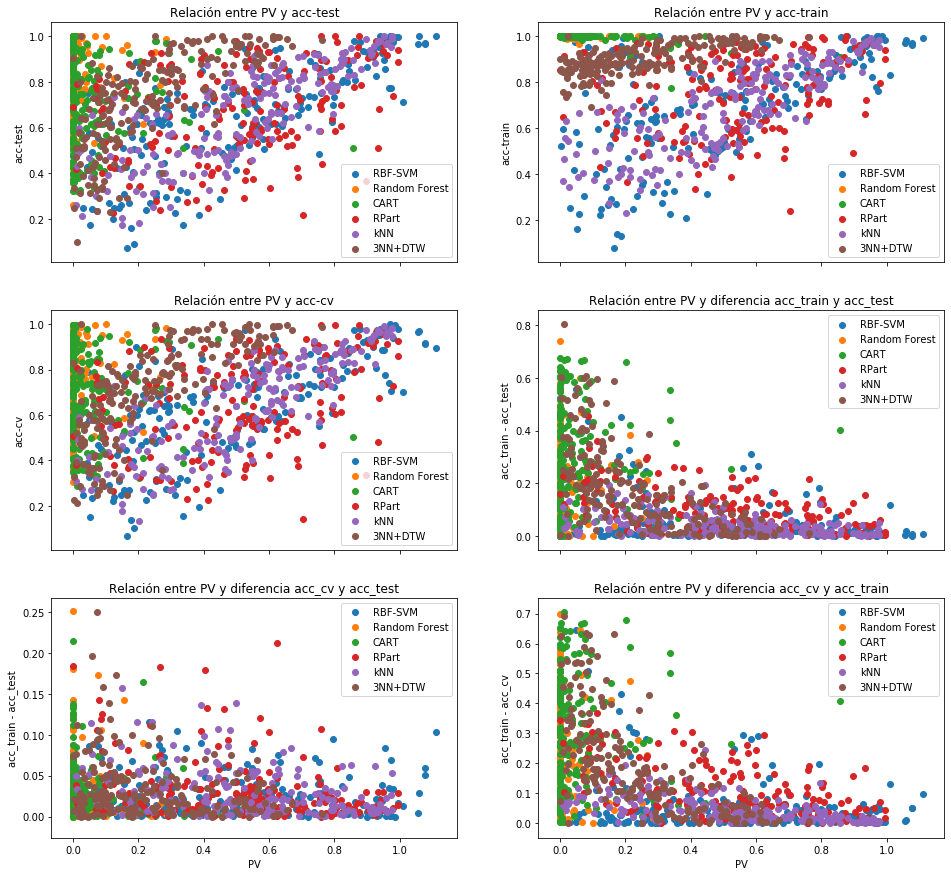
\includegraphics[width=1.2\textwidth]{grupo1}
  \caption{Resultados del grupo 1.}
  \label{fig:pv-grupo1}
\end{figure}

\begin{figure}[htbp]
  \centering
  \hspace*{-1cm}
  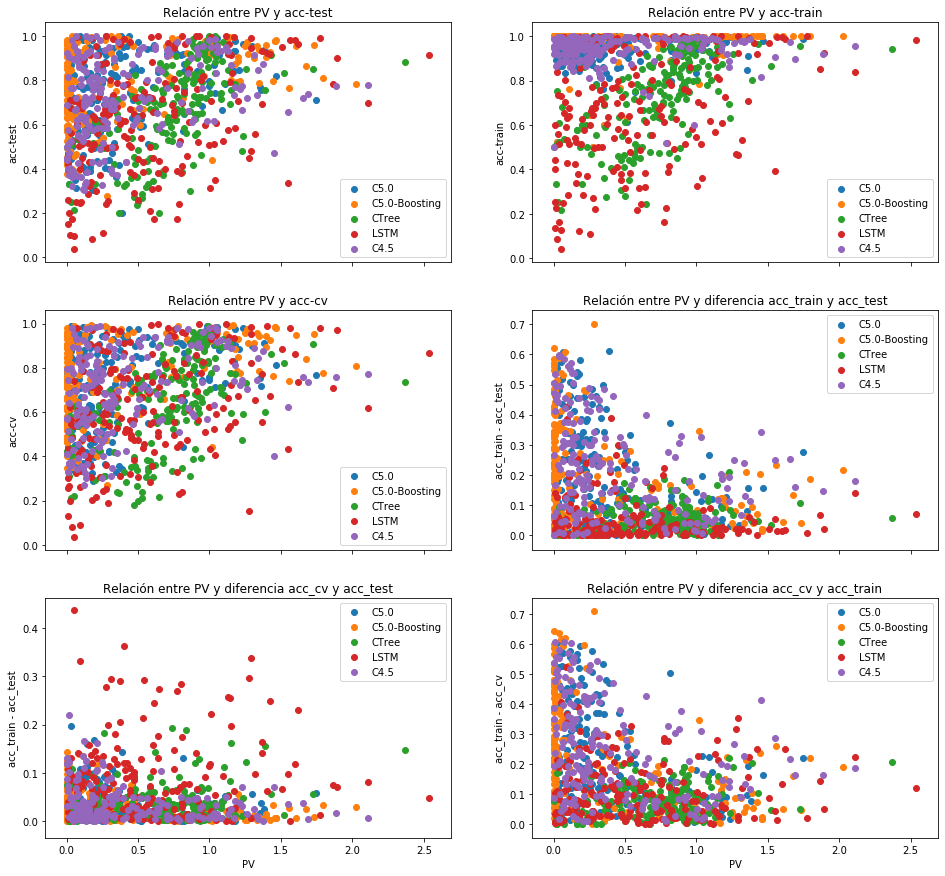
\includegraphics[width=1.2\textwidth]{grupo2}
  \caption{Resultados del grupo 2 (la escala ha cambiado).}
  \label{fig:pv-grupo2}
\end{figure}

En ambos grupos, como ya veníamos viendo de los resultados globales, se mantienen las relaciones del $PV$ que habíamos comentado, sin embargo vemos como el grupo 1 muestra unos resultados más estables:

\begin{itemize}
  \item Excepto 5 valores que están en $[1, 1.1]$, todos los valores $PV$ se encuentran en el intervalo esperado $[0,1]$.
  \item La correlación entre $PV$ y $acc_{test}$ es muy fuerte para SVM, RPart y $k$-NN, donde los datos forman casi una recta de pendiente 1. Para DTW se toma también la tendencia pero con una curva arqueada.
  \item En el caso de Random Forest y CART se nota mucho más el \textbf{fuerte sobreajuste} a los que tienden estos modelos que obtienen valores muy pequeños de $PV$, propiciando valores perfectos de $acc_{train}$ pero muy dispersos en $acc_{test}$.
\end{itemize}

En el grupo 2 vemos unos resultados parecidos en general aunque aquí ya se observan los valores atípicos más frecuentes, que llegan incluso por encima de 2. De hecho los datos de LSTM presentan valores peores (puntos con $PV$ altos pero $acc_{test}$ bajos, sobreajustes muy por encima de los normales) probablemente de una alta varianza que obtenga soluciones inestables. También sea efecto de usar una configuración y entrenamiento fijados para un montón de modelos diferentes, ya que las redes neuronales necesitan estudiar si el entrenamiento está siendo adecuado y converge a una solución correctamente.

Para acabar, resumamos lo obtenido: nuestras hipótesis sobre el $PV$ se cumplen, si bien parece que hay ciertos modelos como el LSTM que pueden presentar una mayor inestabilidad a la hora de obtener el $PV$ por lo que habría que tener cuidado y comprobar que se calcula correctamente. No podemos considerar sustituir la selección clásica con el $PV$ ya que como hemos visto, no tiene por qué tomar el mejor modelo en base al menor error en una muestra distinta. Sin embargo sí podemos utilizarlo como \textbf{selección complementaria}, ayudándonos a hacer una criba más entre modelos con rendimientos muy parecidos asegurándonos así de que escogemos un modelo que ha aprendido mejor \textbf{la relación de los datos}.

\section{Hiperparametrización}

\subsection{Descripción}

\subsubsection{Objetivos}

Comprobada la utilidad de la heurística $PV$, en el contexto de la elección de los \textbf{mejores hiperparámetros} de un modelo es especialmente útil ya que normalmente nos encontramos con muchos valores para los que los modelos obtienen un $acc_{cv}/acc_{test}$ \textbf{muy parecidos} mientras que la complejidad va cambiando. Esto es de especial interés, ya que lo ideal es buscar un modelo con un buen ajuste y que generalice lo mejor posible para evitar tiempos de computación innecesarios y sobreajustes que pudieran darse.

Buscaremos así  si $PV$ destaca en la búsqueda de la mejor configuración de hiperparámetros posible para un modelo dado, frente a la métrica clásica $acc_{CV}$. Para ello escogeremos unos cuantos \emph{datasets} y unos cuantos modelos típicos buscando los hiperparámetros óptimos de cada modelo en cada dataset, y veremos cual es el comportamiento entre las métricas frente a la variación de los hiperparámetros.

\subsubsection{Datasets}

Cogemos cuatro \emph{dataset} de "\emph{UEA \& UCR Time Series Classification}" \cite{bagnall2020ts} (\autoref{table:pv-datasets1}, \autoref{table:pv-datasets2}): \emph{ChlorineConcentration}, \emph{PowerCons}, \emph{SmoothSubspace}, \emph{ProximalPhalanxTW}.

\subsubsection{Clasificadores}

Hemos seleccionado cuatro clasificadores de los que habíamos usado en el anterior experimento que tienen hiperparámetros fáciles de comprender. En principio usamos las mismas configuraciones que el anterior experimento, variando solamente los hiperparámetros que comentamos:

\begin{itemize}
  \item \textbf{LSTM}: el espacio de hiperparámetros es el número de neuronas de la capa LSTM donde cuantas más neuronas se tengan más complejo es el modelo. El espacio de búsqueda serán 10 enteros equidistantes en el intervalo $[10, 110]$.
  \item \textbf{SVM}: variamos el hiperparámetro $C$ que nos indica cuanto se permite ignorar el error de clasificación, cuanto más alto menos fallos se permite por lo que baja el error a costa de menor generalización y mayor tiempos de cálculo. Para la búsqueda tomamos 15 puntos equidistantes en el intervalo $[-4, 4]$ como exponentes para $10$ (escala logarítmica).
  \item \textbf{Random Forest}: variamos la profundidad máxima de los árboles que creamos. Cuanto menor sea, los árboles son más simples y tienen mayor error pero reducen la varianza y también los tiempos de cómputo. Tomamos el espacio $\{1, 2, \ldots, 14\}$.
  \item \textbf{$k$-NN}: el hiperparámetro a cambiar es el número de vecinos considerado $k$ que en este caso cuanto más alto mas \emph{simple} será pero añadirá más tiempos de cálculo. Tomamos 20 enteros equidistantes en el intervalo $[2, 60]$ (excluimos el 1 ya que siempre sobreajusta).
\end{itemize}

\subsubsection{Métricas}

Mediremos para cada configuración de cada modelo los siguientes valores:

\begin{itemize}
  \item $PV$: con $n = 5$, $r_1 = 0.1$ y $r_n = 0.3$.
  \item $acc_{CV}$: con 5 particiones.
  \item $acc_{test}$
\end{itemize}

\subsection{Resultados}

Mostramos una imagen por cada modelo, mostrando a la vez los resultados en los cuatro \emph{datasets} donde se han dibujado las tres curvas correspondientes a cada métrica obtenida.

Los resultados se muestran en orden para LSTM (\autoref{fig:hiper-LSTM}), SVM (\autoref{fig:hiper-SVM}), Random Forest (\autoref{fig:hiper-RF}) y $k$-NN (\autoref{fig:hiper-KNN}).

\begin{figure}[htbp]
  \centering
  \hspace*{-1cm}
  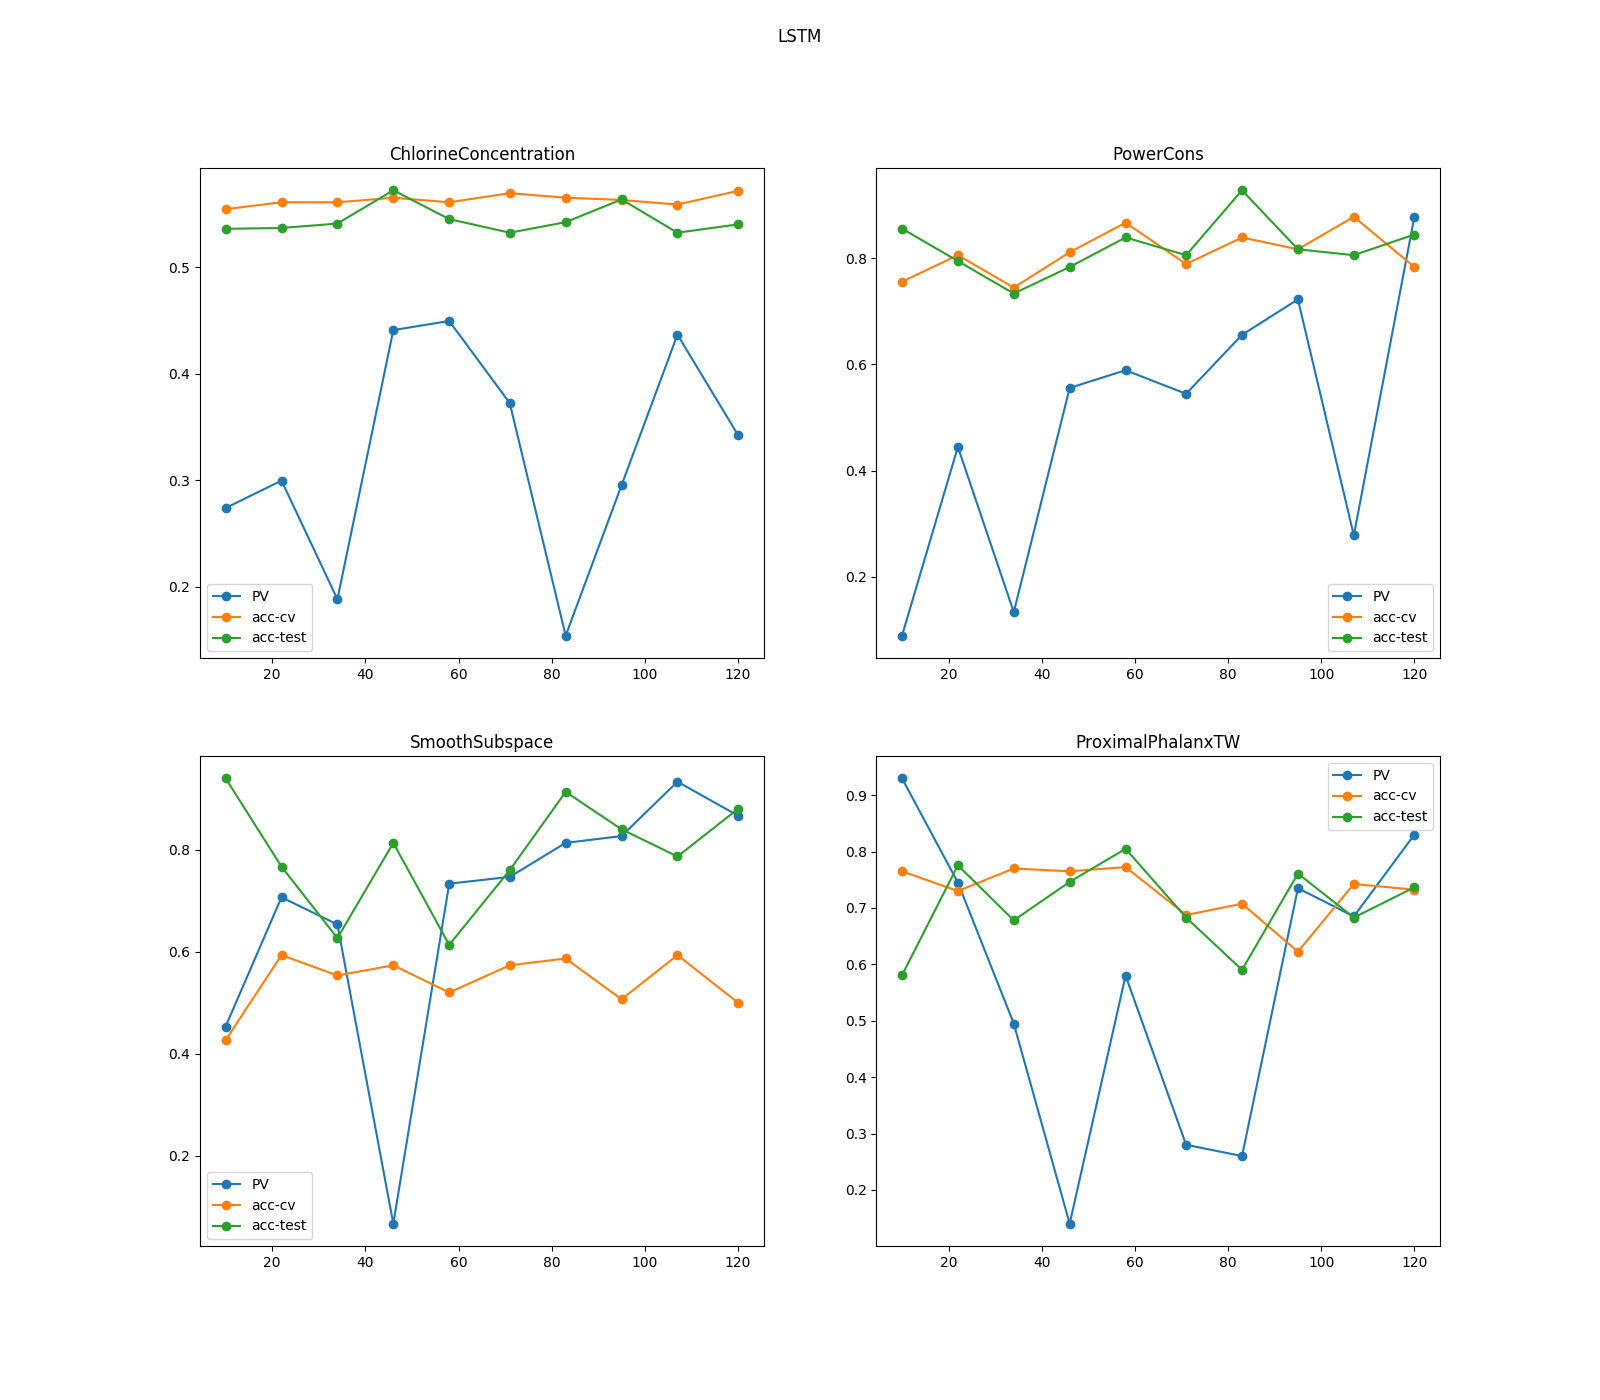
\includegraphics[width=1.2\textwidth]{hiper_LSTM}
  \caption{Resultados hiperparámetros LSTM.}
  \label{fig:hiper-LSTM}
\end{figure}

\begin{figure}[htbp]
  \centering
  \hspace*{-1cm}
  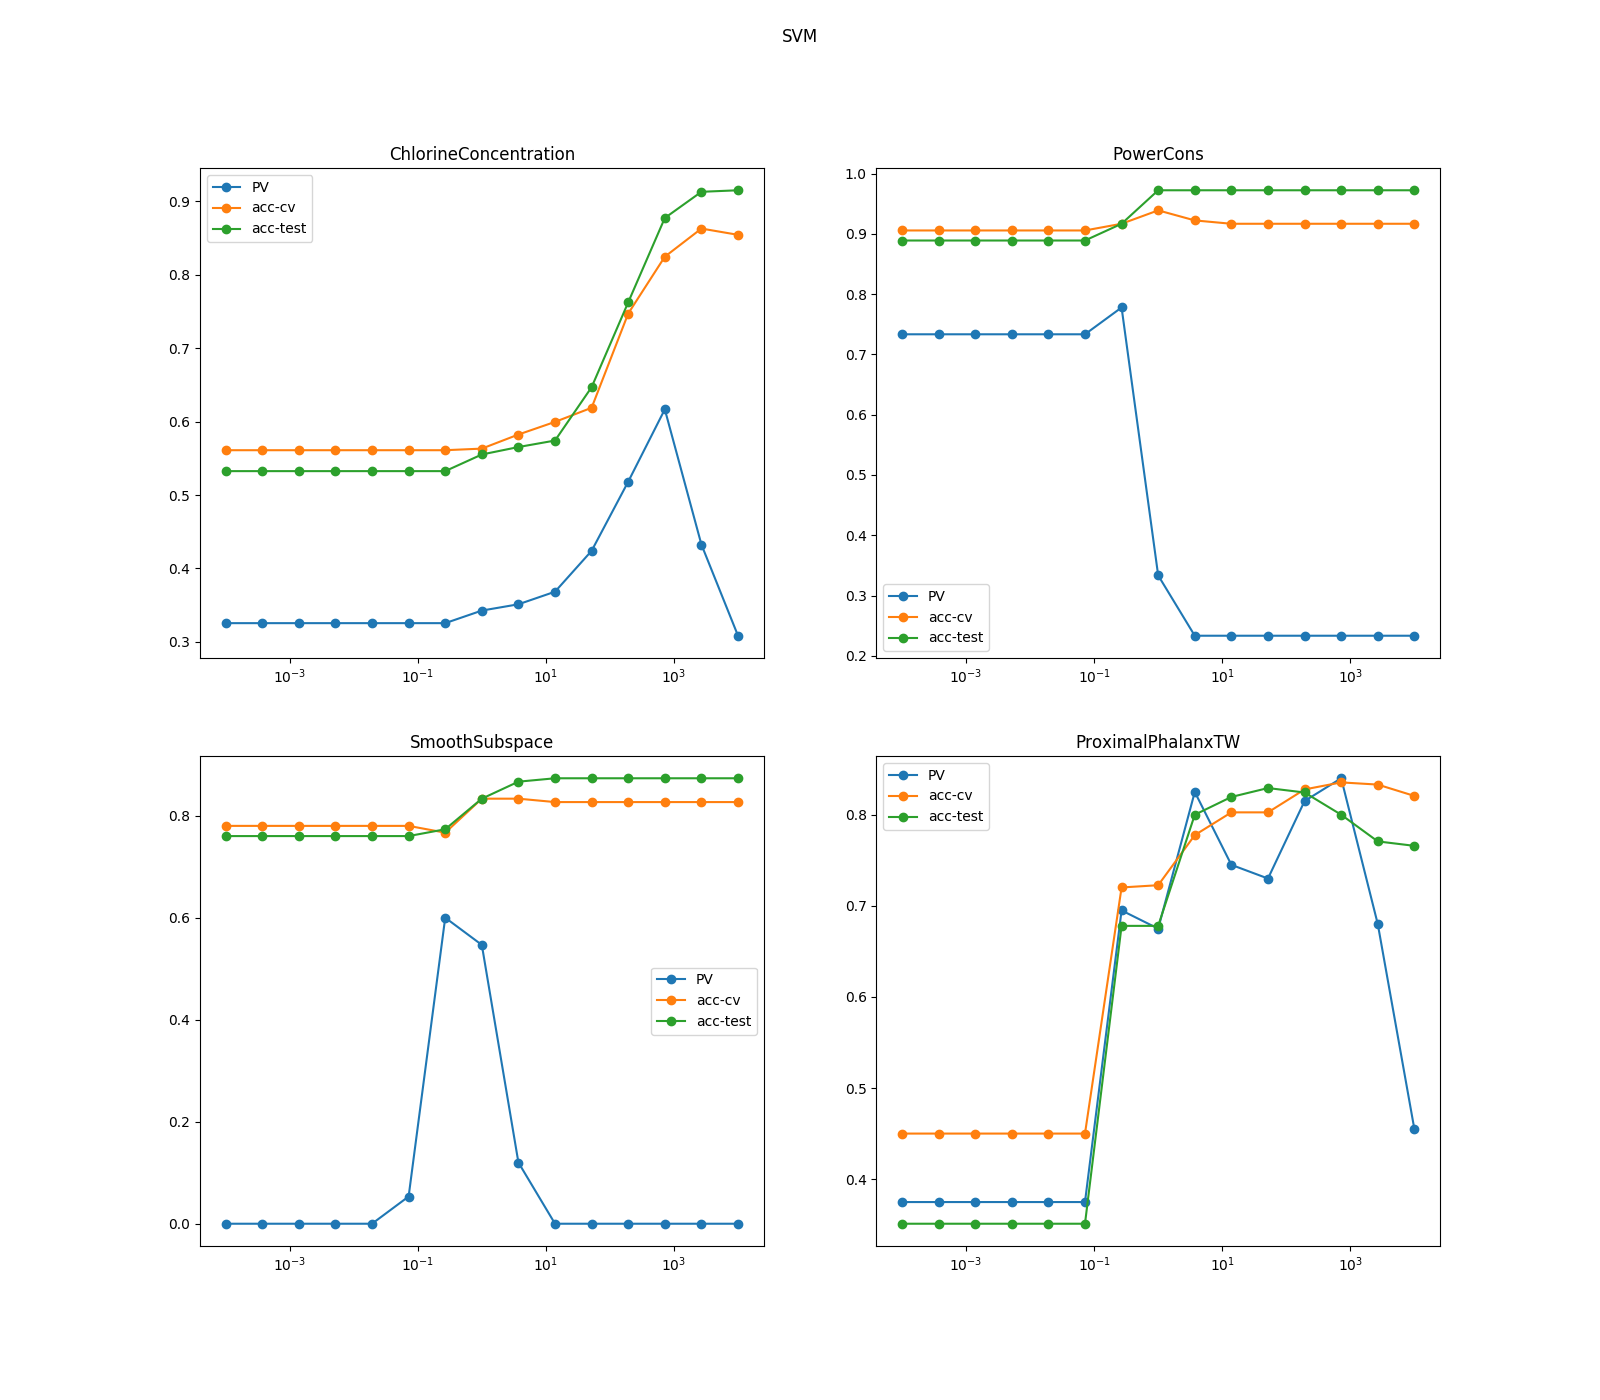
\includegraphics[width=1.2\textwidth]{hiper_SVM}
  \caption{Resultados hiperparámetros SVM.}
  \label{fig:hiper-SVM}
\end{figure}

\begin{figure}[htbp]
  \centering
  \hspace*{-1cm}
  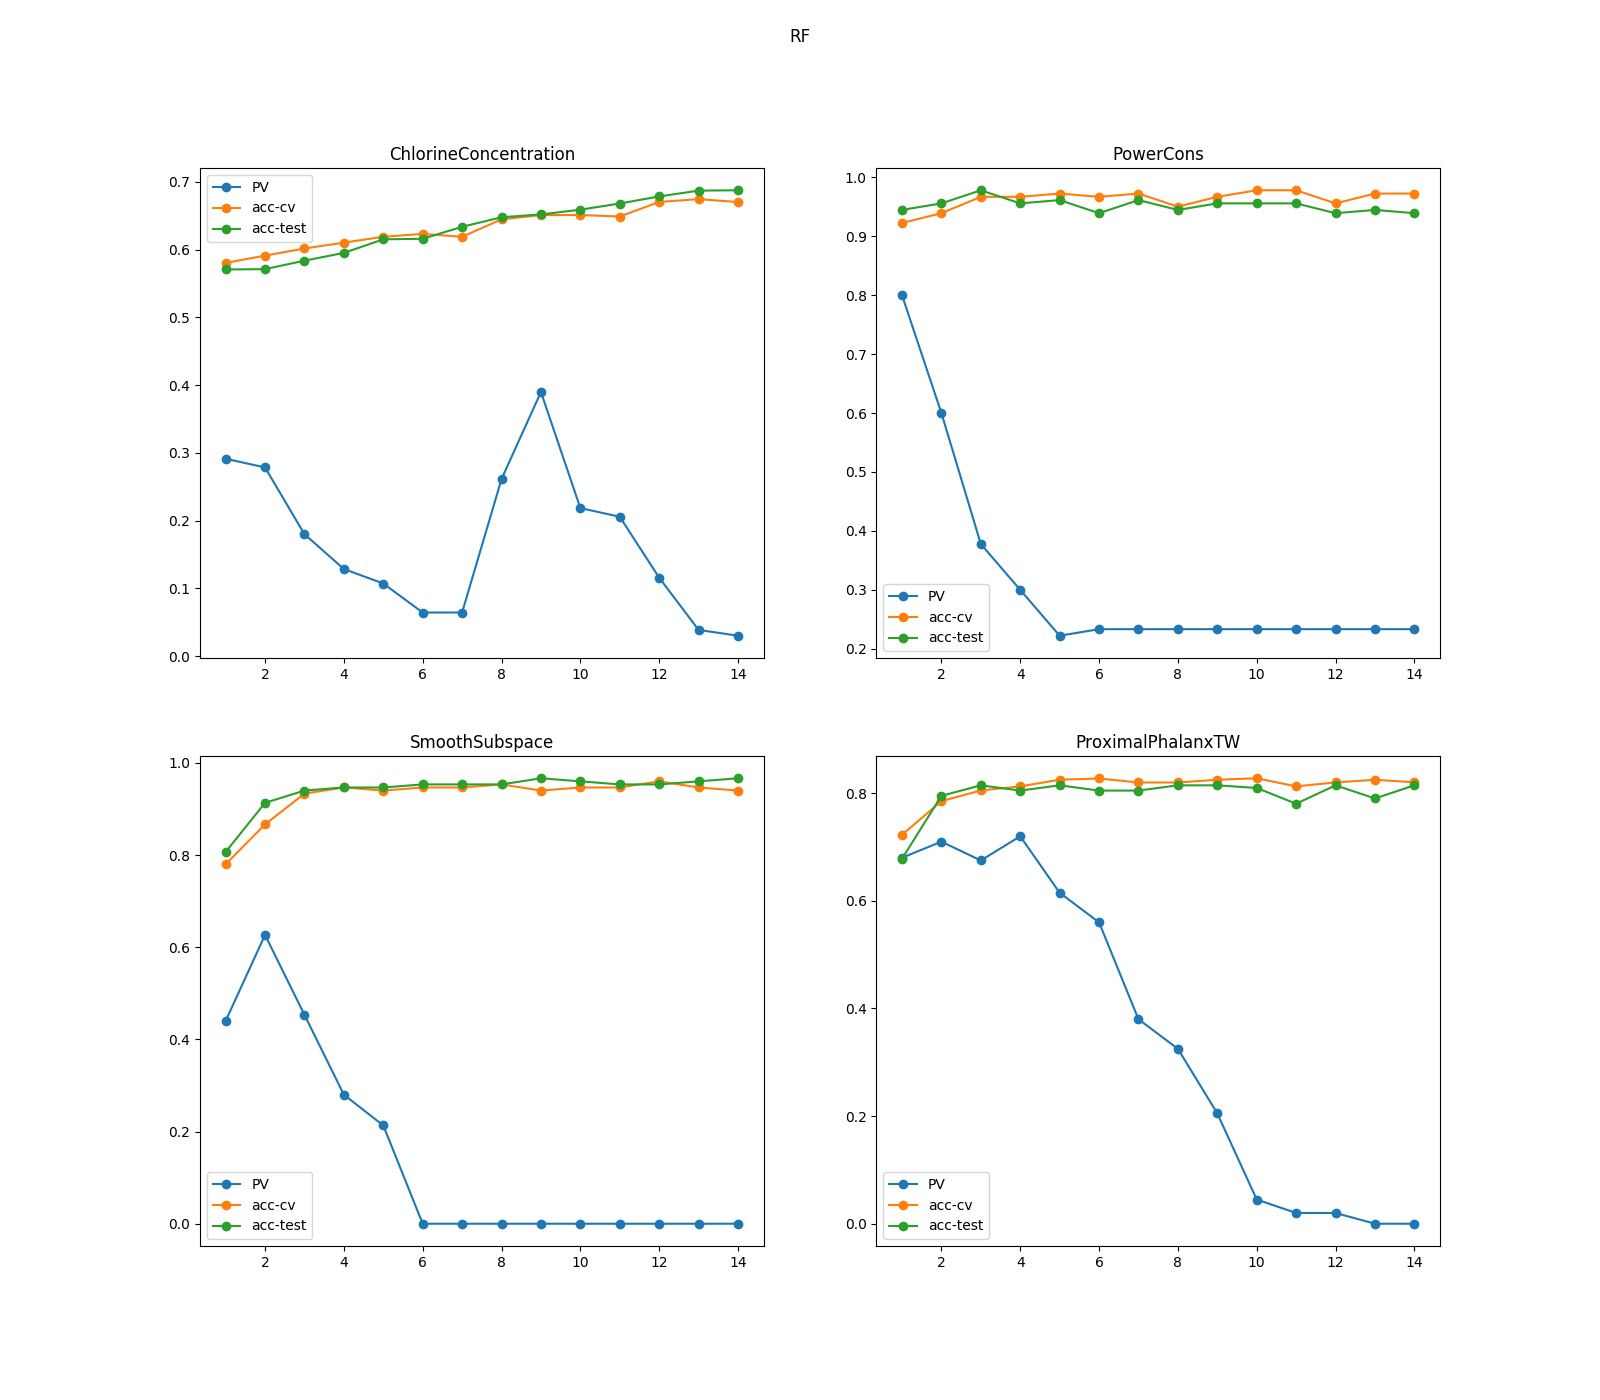
\includegraphics[width=1.2\textwidth]{hiper_RF}
  \caption{Resultados hiperparámetros Random Forest.}
  \label{fig:hiper-RF}
\end{figure}

\begin{figure}[htbp]
  \centering
  \hspace*{-1cm}
  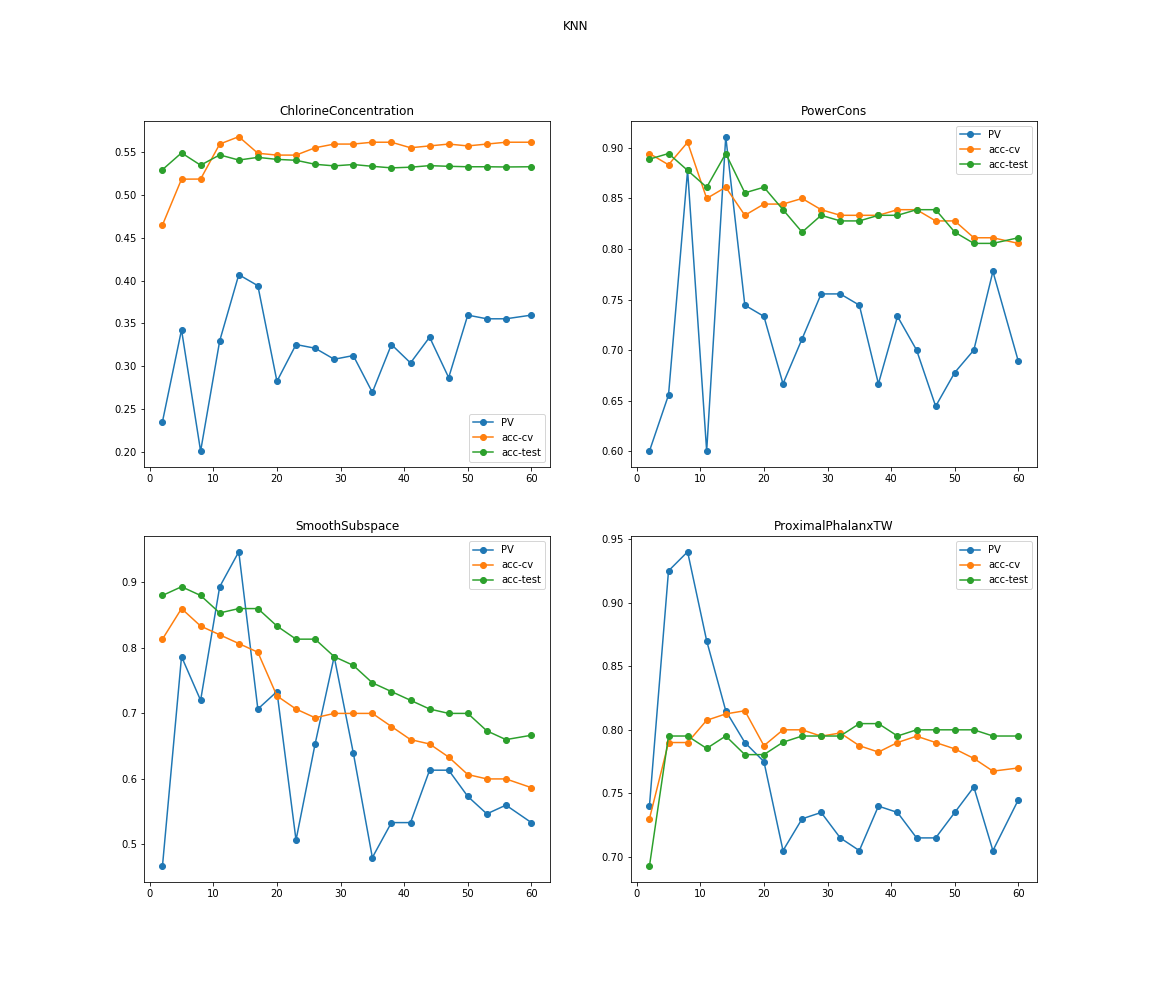
\includegraphics[width=1.2\textwidth]{hiper_KNN}
  \caption{Resultados hiperparámetros $k$-NN.}
  \label{fig:hiper-KNN}
\end{figure}

\subsection{Análisis}

Primero analicemos los resultados modelo a modelo. Para LSTM observamos que en los 4 \emph{datasets} para $acc_{CV}$ se obtienen valores muy similares donde no hay ninguno que resalte especialmente, mientras que $PV$ presenta una mayor variación. Además los valores más grandes de $PV$ parecen ir ligados con los más altos de $acc_{test}$ aunque habría que tener cuidado, debido a la posible inestabilidad que habíamos comentado sobre el modelo LSTM.

En SVM, las curvas obtenidas aquí son más \emph{suaves} y vemos como $PV$ capta bien los cambios importantes de acierto: cuando las métricas empiezan a cambiar substancialmente, esto se refleja con un crecimiento en el $PV$ pero a diferencia de las métricas que vuelven a estabilizarse, $PV$ vuelve a decrecer. En todo caso parece que los valores máximos del $PV$ parecen coincidir con las métricas clásicas, pero en cuanto el modelo es muy complejo o simple se castiga con valores bajos.

Para Random Forest pasa algo muy parecido a SVM: en este caso las métricas clásicas van unidas pero no se da ningún valor al hecho de que estamos aumentando innecesariamente la profundidad y por tanto, la complejidad del modelo. $PV$ es capaz él solo de determinar cual es el hiperparámetro óptimo que nos da el mejor rendimiento sin pasarse de complejidad.

En $k$-NN tenemos unas curvas de $PV$ más \emph{espinosas} pero se repiten los mismos hechos que hemos observado.

Recapitulando, vemos que $PV$ es capaz de \textbf{discriminar} mejor que $acc_{CV}$ permitiendo considerar no solo el buen ajuste del modelo sino también la complejidad del modelo donde $acc_{CV}$ puede mantener valores iguales. Además los valores máximos de $PV$ se parecen corresponder con los máximos de $acc_{test}$ más o menos y que pudiera reemplazarse directamente por $acc_{CV}$, pero también se pueden usar \textbf{conjuntamente} para tener una mayor seguridad si se quiere obtener el mejor ajuste posible. Finalmente confirmamos la relación del anterior experimento de a mayor $PV$, mayor $acc_{test}$.

\endinput
